\documentclass{article}

% ---------------------------------------------------------------
% NeurIPS 2026 Evaluations & Datasets Track (double-blind)
% The track was renamed from "Datasets & Benchmarks" to
% "Evaluations & Datasets" for 2026.  The .sty ships [dandb];
% switch to [eandd] if/when the template adds it.
% ---------------------------------------------------------------
\usepackage[dandb]{neurips_2026}
% Camera-ready: \usepackage[dandb, final]{neurips_2026}
% Note: track renamed to E&D for 2026 but .sty still uses [dandb]; verified 2026-04-17.

\usepackage[utf8]{inputenc}
\usepackage[T1]{fontenc}
\usepackage{hyperref}
\usepackage{url}
\usepackage{booktabs}
\usepackage{amsfonts}
\usepackage{nicefrac}
\usepackage{microtype}
\usepackage{xcolor}
\usepackage{graphicx}
\usepackage{amsmath}
\usepackage{enumitem}       % for [leftmargin=*]
\usepackage{multirow}       % for multi-row table cells
\usepackage{subcaption}     % for subfigures
\usepackage{wrapfig}        % optional: for wrapped figures
\usepackage{pifont}          % for \ding{55} (cross mark)

%%%%%%%%%%
% RPX brand palette
\definecolor{rpxR}{HTML}{4F46E5}  % indigo-600
\definecolor{rpxP}{HTML}{DB2777}  % pink-600
\definecolor{rpxX}{HTML}{C2410C}  % orange-700
\newcommand{\coolname}{\textsc{\textcolor{rpxR}{R}\textcolor{rpxP}{P}\textcolor{rpxX}{X}}}
\newcommand{\coolnamedetect}{\coolname-\textit{Detector}}
\newcommand{\coolabbrdetect}{\textit{CG-D}}
% Anonymised for submission; restore for camera-ready
\newcommand{\webpage}{https://anonymous.4open.science/r/RPX}
\newcommand{\authorhref}[3][flodarkpurple]{\href{#2}{\color{#1}{#3}}}
\newcommand{\authorspace}{\hspace{.95em}}
\newcommand{\todo}[1]{\textcolor{red}{TODO: #1}}
\newcommand{\finding}[1]{\textcolor{blue}{\textbf{Finding:} #1}}
\newcommand{\cmark}{\textcolor{green!70!black}{\checkmark}}
\newcommand{\xmark}{\textcolor{red!80!black}{\ding{55}}}
\newcommand{\pmark}{\textcolor{orange!80!black}{$\circ$}}
%%%%%%%%%%

\title{Same Scene, Different Story: How Well Do Pretrained Perception Models Actually Work on Robots?

% Alternatives considered:
% Same Scene, Different Story: Ranking Robot Perception Backbones for Real-World Deployment
% Same Scene, Different Story: Pretrained Perception Models Fail Where Robots Need Them Most (use if finding confirms)
}

% Double-blind: anonymous
\author{Anonymous Author(s)}

\begin{document}

\maketitle

\vspace{-2em}

\begin{figure}[h!]
    \centering
    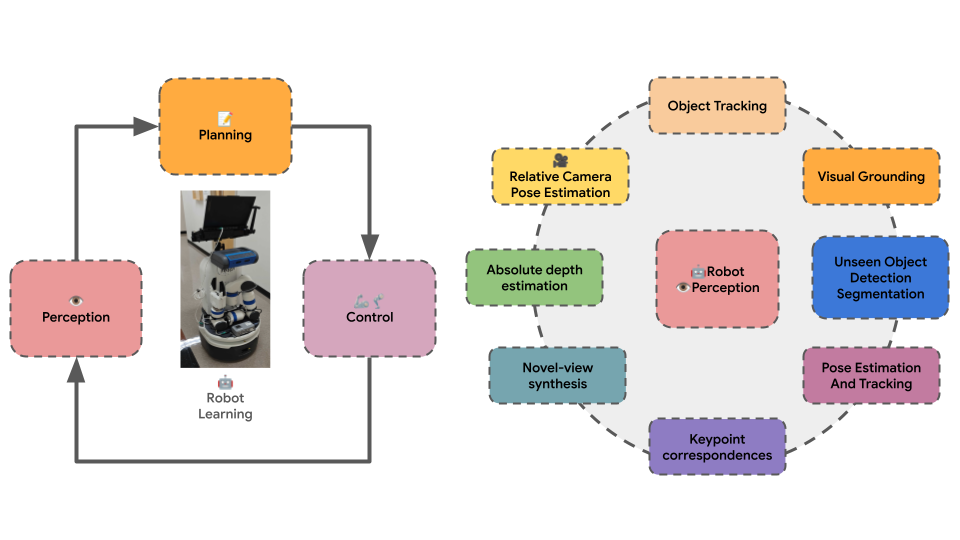
\includegraphics[width=.95\linewidth]{assets/images/RPX-overview.png}
    \vspace{-.5em}
    \caption{\coolname{} framework overview.
    A human-carried rig (D435 RGB-D + T265 6-DoF pose + GoPro ego) captures 100 real-world scenes under a three-phase protocol (clutter $\to$ interaction $\to$ clean).
    Five perception tasks (\S\ref{sec:tasks}) are evaluated on identical scenes and objects; the dataset additionally supports tasks shown in the figure but not evaluated in this work (\S\ref{sec:conclusion}).
    Deployment-readiness metrics (TS, STR, SGC) and Effort-Stratified Difficulty (ESD) reveal how foundation models perform under embodied deployment conditions---not just on static accuracy.}
    \label{fig:main-figure}
\end{figure}

\vspace{-1em}

\begin{abstract}
Pretrained perception models---depth estimators, object detectors, trackers, and vision-language models---are now standard components in robot learning systems, yet the choice of which model to deploy is made without evidence from the conditions robots actually face.
Standard benchmarks use curated internet images; robots see the world through low-resolution Intel RealSense sensors under clutter, hand occlusion, motion blur, and challenging surfaces.
We introduce \coolname{}, a real-world evaluation methodology and benchmark that quantifies the \textit{deployment readiness} of pretrained perception models for embodied robotics.
%
A human carrying the same sensor rig a mobile robot would use (D435 RGB-D + T265 tracking + GoPro egocentric) captures 100 scenes spanning indoor and outdoor environments, daylight and night, reflective and transparent surfaces, across ${\sim}$70 object categories and 75{,}000 frames.
%
Each scene is captured in three phases that mirror the robot manipulation cycle:
\textbf{clutter} (the scene as a robot naturally finds it),
\textbf{interaction} (a human manipulates objects---the data that learning-from-humans pipelines train on), and
\textbf{clean} (the scene reorganised---the condition models are designed for).
%
The gap between clean-scene and clutter/interaction performance \textit{is} the deployment readiness gap, and no existing benchmark measures it.
%
\coolname{} evaluates \todo{N} models across \todo{M} perception tasks on the \textit{same} physical scenes and objects, using deployment-readiness metrics---State-Transition Robustness, Geometric Coherence, and Effort-Stratified Difficulty---that capture properties invisible to static accuracy and compose into an Embodied Deployment Score (EDS).
%
\todo{HEADLINE FINDING.}
%
\coolname{} is released as a pip-installable, bring-your-own-model toolkit at \url{\webpage}.
\end{abstract}

\section{Introduction}
\label{sec:intro}

\noindent
What the robot fails to see, it fails to do.
Modern robot learning places large pretrained perception models at this first point of contact with the physical world.
Vision-Language-Action (VLA) models ($\pi_0$~\citep{black2024pi0}, OpenVLA~\citep{kim2024openvla}, GR00T~\citep{bjorck2025gr00t}) inherit visual encoders from Vision-Language Models (VLMs) such as SigLIP~\citep{zhai2023siglip} and DINOv2~\citep{oquab2023dinov2}.
Modular systems chain open-vocabulary detectors (GroundingDINO~\citep{liu2024groundingDINO}), segmenters (SAM2~\citep{ravi2024sam2}), and depth models (ZoeDepth~\citep{bhat2023zoedepth}) for grasp planning~\citep{liu2024okrobot, ze2024dp3}.
World models (TesserAct~\citep{zhen2025tesseract}) consume and generate depth and normal maps conditioned on actions.
In each case, perception quality strongly influences downstream success.

\paragraph{The unjustified backbone choice.}
Despite this dependence, backbone selection is ad hoc.
Li~et~al.~\citep{li2025robovlms} confirmed that visual backbone choice dominates VLA policy success---more than architecture or training recipe---but evaluated entirely in simulation.
OK-Robot~\citep{liu2024okrobot} showed that perception quality is the dominant bottleneck in real-world pick-and-place (success drops from 82\% to 59\% under clutter), but evaluated only one perception pipeline without comparing alternatives.
The problem is not a lack of models---it is a lack of evidence about which model to use.
Three deficiencies in current evaluation keep the choice unjustified.
\textbf{(i)~Sensor mismatch:} models are ranked on COCO~\citep{lin2014coco} and ImageNet~\citep{deng2009imagenet}---curated internet images at high resolution. Robots see through \$30 Intel RealSense D435 sensors at $640\!\times\!480$ with structured-light depth noise, motion blur, and specular artifacts. No benchmark evaluates models on this imagery.
\textbf{(ii)~Task silos:} each task is evaluated on a different benchmark with different scenes, so per-task leaderboards cannot compose into a deployment recommendation.
\textbf{(iii)~No scene-state variation:} existing benchmarks capture static scenes. A robot's scene changes as it acts---objects move, hands occlude, clutter shifts. No benchmark measures how perception degrades during manipulation and whether it recovers afterward.

\paragraph{Evaluation methodology, not just a dataset.}
The 2026 NeurIPS E\&D track asks: \textit{what claims does an evaluation support, under what assumptions?}
We argue that answering ``which perception backbone should a robot use?'' requires \textbf{evaluation methodology} that existing benchmarks lack---not more data, but better measurement.
Specifically, evaluation must:
(a)~create controlled scene-state variation so that performance differences are primarily attributable to scene state, not confounded by object or lighting changes;
(b)~measure properties beyond accuracy---temporal consistency, phase-transition robustness, geometric coherence---that determine whether a model \textit{works in deployment};
and (c)~stratify difficulty by perceptual ambiguity, not post-hoc geometry.

\paragraph{\coolname{}: methodology + dataset + toolkit.}
We introduce \coolname{}, which provides all three.
The \textit{three-phase capture protocol} (\S\ref{sec:three-phase}) mirrors the robot manipulation cycle (observe $\to$ act $\to$ verify), holding scene identity fixed while varying scene state.
\textit{Effort-Stratified Difficulty} (\S\ref{sec:features}) derives difficulty from annotation effort---a direct signal of perceptual ambiguity.
Three \textit{deployment-readiness metrics} (\S\ref{sec:deploy-metrics})---Temporal Stability (TS), State-Transition Robustness (STR), and Geometric Coherence (SGC)---compose into an Embodied Deployment Score (EDS, \S\ref{sec:eds}) that ranks models for real-world use.
These are instantiated on a 75{,}000-frame real-world RGB-D corpus across 100 scenes and ${\sim}$70 object categories (\S\ref{sec:dataset}).
All five tasks---depth, detection/grounding, tracking, scene QA, spatial QA---are evaluated on the \textit{same} scenes and objects, described in crowd-sourced natural language~\citep{padalunkal2023fewsol}, with a pip-installable toolkit (\S\ref{sec:toolkit}) that enables reproducible bring-your-own-model evaluation.

\paragraph{Human proxy for robot perception.}
A human carries the exact sensor rig a mobile robot would use---D435 (RGB-D at $640\!\times\!480$) + T265 (stereo tracking) + GoPro (egocentric)---through 100 real-world scenes: kitchens, offices, outdoor paths, staircases, day and night, reflective and transparent surfaces.
This is not a limitation but a deliberate design: the learning-from-humans paradigm~\citep{padalunkal2024iteach, 2025hrt1, khazatsky2024droid, kareer2024egomimic} already uses human-captured video as robot training data.
If pretrained models fail on human-captured RealSense imagery, they fail on the data robots are trained on.
Paired single-object and multi-object scenes enable controlled comparison of text-prompted vs.\ image-prompted perception under real-world conditions.

% ── TODO(results): replace once experiments complete ──
\paragraph{Key findings.}
Evaluating \todo{N} models across five tasks, we find:
\todo{REPLACE with 2--3 concrete findings. Candidates:
(i) static accuracy is weakly correlated with deployment robustness ($\rho = X$);
(ii) model rankings on Hard scenes diverge from Easy ($\tau = X$);
(iii) VLM spatial QA accuracy drops by X\% during interaction, directly implicating VLA backbone robustness;
(iv) EDS predicts downstream grasp success ($\rho = X$).}

\paragraph{Contributions.}
\begin{enumerate}[leftmargin=*, topsep=2pt, itemsep=1pt]
    \item \textbf{An evaluation methodology for deployment-ready robot perception.}
    Three-phase protocol + ESD + task-specific deployment-readiness metrics (TS, STR, SGC) + EDS---a methodological framework that can be applied to future datasets and tasks beyond \coolname{}.

    \item \textbf{The RPX dataset and multi-task benchmark.}
    75{,}000-frame real-world RGB-D corpus across 100 scenes and ${\sim}$70 object categories, with five perception tasks (depth, detection/grounding, tracking, scene QA, spatial QA) evaluated on the \textit{same} scenes and objects---enabling the first cross-task deployment recommendations on shared real-world scenes.

    \item \textbf{Empirical findings.}
    \todo{2--3 sentence findings summary, including the named finding.}

    \item \textbf{Self-sustaining community toolkit.}
    \texttt{rpx-benchmark}: pip-installable, bring-your-own-model, with plugin registries for new tasks and metrics. 138 CI-verified tests.
\end{enumerate}

\paragraph{Scope.}
\coolname{} tests the claim that pretrained perception backbones differ in deployment robustness in ways not predictable from standard accuracy alone.
It evaluates perception at the output level (depth maps, boxes, QA answers); for VLAs that consume encoder features, output-level metrics serve as proxies for feature quality (justified in \S\ref{sec:eds}, validated in \S\ref{sec:downstream}).
Assumptions and scope limitations are detailed in Appendix~\ref{sec:appendix-scope}.

\section{Related Work}\label{sec:related}

\coolname{} addresses a gap at the intersection of six bodies of work: foundation models in robot learning stacks, vision-language-action (VLA) models and world models, robot perception datasets, embodied benchmarks, robustness and difficulty stratification, and in-context visual prompting for robotics.
Table~\ref{tab:dataset-comparison} provides a systematic comparison across 14 dimensions.

%% ── 1. Foundation models in robot perception ──
\paragraph{Foundation models as perception substrates for robot learning.}
Large pretrained vision models now occupy three distinct roles in robot manipulation.
%
\textit{As frozen visual backbones for policy learning}, DINOv2~\citep{oquab2023dinov2} and SigLIP~\citep{zhai2023siglip} provide the visual features that VLA models (OpenVLA~\citep{kim2024openvla}, $\pi_0$~\citep{black2024pi0}, GR00T~N1~\citep{bjorck2025gr00t}) consume to predict actions.
The choice of visual encoder strongly shapes what the policy ``sees,'' yet it is typically inherited from the underlying VLM (e.g., PaliGemma $\to$ SigLIP in $\pi_0$) without independent evaluation on robot-relevant scenes.
%
\textit{As perception preprocessors in modular systems}, GroundingDINO~\citep{liu2024groundingDINO}, SAM2~\citep{ravi2024sam2}, and monocular depth models feed signals into grasp planners, object trackers, and navigation stacks.
OK-Robot~\citep{liu2024okrobot} is a paradigmatic example: it chains Lang-SAM, AnyGrasp, and a navigation planner for zero-shot pick-and-place in 10 real homes.
Its analysis reveals that \textit{perception quality is the primary bottleneck}: success drops from 82\% in clean environments to 59\% in cluttered ones, with perception failures (missed detections, poor segmentation) identified as the dominant cause~\citep{liu2024okrobot}---yet neither OK-Robot nor any other deployed system systematically compares the available perception backbones.
%
\textit{As pseudo-ground-truth generators}, ZoeDepth~\citep{bhat2023zoedepth} creates the 3D point clouds that 3D Diffusion Policy~\citep{ze2024dp3} trains on; ZoeDepth is also used to augment GR-1/GR00T fine-tuning with synthetic depth for embodiments lacking depth sensors.
Inaccuracies in these pseudo-labels can propagate into the learned policy.

SceneReplica~\citep{scenereplica} benchmarks real-world pick-and-place with swappable perception modules and confirms that perception dominates end-to-end success, but evaluates only 20 tabletop scenes without temporal dynamics or multi-task coverage.
Open-X Embodiment~\citep{open_x_embodiment_rt_x_2023} aggregates demonstration data at scale but focuses on action learning, not perception ranking.
\coolname{} is, to our knowledge, the first benchmark whose explicit purpose is to rank perception backbones across multiple tasks on the same real-world scenes.

%% ── 2. VLAs and world models ──
\paragraph{VLAs, world models, and the backbone selection problem.}
The recent surge in VLA models---from RT-1/RT-2~\citep{brohan2023rt2} through Octo~\citep{ghosh2024octo} to $\pi_0$~\citep{black2024pi0}, OpenVLA~\citep{kim2024openvla}, and GR00T~\citep{bjorck2025gr00t}---and embodied world models~\citep{zhen2025tesseract} has made the visual backbone choice more consequential than ever.
Li~et~al.~\citep{li2025robovlms} directly study this in ``What matters in building VLAs for generalist robots'' (Nature Machine Intelligence): they systematically compare DINOv2, SigLIP, CLIP, and fusion strategies as VLA backbones and find that \textit{backbone choice is the dominant factor in policy success}---more important than architecture or training recipe.
However, their evaluation is conducted entirely in simulation (SimplerEnv, CALVIN), where the structured-light depth noise, motion blur, specular reflections, and hand occlusion dynamics of real deployment are absent.
Crucially, because they evaluate end-to-end policy success, they \textit{cannot decompose} whether a failure is due to perception or policy---a confound that perception-level evaluation resolves.

Embodied world models (TesserAct~\citep{zhen2025tesseract}, GWM~\citep{lu2025gwm}) predict future RGB, depth, and normal frames conditioned on actions.
Reward models increasingly rely on visual perception: VIP~\citep{ma2023vip} pre-trains visual reward functions from human video; ReWiND~\citep{zhang2025rewind} uses language-conditioned VLM rewards for task adaptation; Robometer~\citep{liang2026robometer} scales reward models across 1M+ trajectories with video-language understanding.
These models consume perception signals (depth, segmentation) as training inputs and generate them as outputs; their quality is bounded by the fidelity of the underlying perception.
Yet no existing benchmark evaluates whether these perception signals are \textit{robust enough} under the deployment conditions the downstream systems will encounter.
\coolname{} provides exactly this evaluation: if ZoeDepth's metric accuracy degrades by $X$\% during human interaction (as measured by STR), any world model or policy trained on ZoeDepth pseudo-labels inherits that degradation.

%% ── 3. Robot perception datasets ──
\paragraph{Robot perception datasets.}
Existing datasets each cover a fragment of the evaluation space \coolname{} targets.
\textbf{Object pose:} YCB-Video~\citep{xiang2018posecnn} and BOP~\citep{hodan2024bop} provide 6-DoF pose for known objects with static cameras; SenseShift6D~\citep{han2025senseshift6d} adds sensor-variation robustness but covers only 5 objects.
\textbf{Segmentation:} OCID~\citep{suchi2019ocid} captures cluttered tabletops but has no temporal dynamics or camera pose; RISeg~\citep{qian2024riseg} uses robot interaction for segmentation without comparative backbone evaluation.
\textbf{Reconstruction:} ScanNet~\citep{dai2017scannet}, HM3D~\citep{ramakrishnan2021hm3d}, and EmbodiedScan~\citep{wang2024embodiedscan} provide multi-modal 3D data but target reconstruction/navigation, not manipulation perception, and have no phase structure.
\textbf{Human activity:} EPIC-Kitchens~\citep{damen2018epic} and RH20T~\citep{fang2023rh20t} contain interaction video but lack the instance masks, metric depth, and camera pose required for perception evaluation.
\textbf{Robot-relevant objects:} FewSOL~\citep{padalunkal2023fewsol} and NIDS-Net~\citep{lu2025nidsnet} study recognition on daily objects but not multi-task evaluation.
\textbf{Large-scale robot data:} DROID~\citep{khazatsky2024droid} aggregates 76K real-world manipulation trajectories across 564 scenes with multi-camera views, but targets policy learning rather than perception ranking---it provides no per-frame perception ground truth (depth, masks) or deployment-readiness metrics.

\textit{No prior dataset evaluates multiple perception tasks on the same scenes and the same objects}---the confound that prevents per-task leaderboards from composing into a deployment recommendation.

%% ── 4. Embodied and multi-task benchmarks ──
\paragraph{Embodied and multi-task benchmarks.}
AI2-THOR~\citep{kolve2017ai2thor}, Habitat~\citep{savva2019habitat}, HomeRobot~\citep{yenamandra2023homerobot}, BEHAVIOR-1K~\citep{li2023behavior1k}, and BEHAVIOR Vision Suite~\citep{ge2024behavior} enable multi-task evaluation in simulation---the latter with customisable scene generation---but cannot replicate real-world sensing (structured-light noise, specular reflections, motion blur).
EmbodiedBench~\citep{yang2025embodiedbench} benchmarks MLLMs as embodied agents but in simulation with action-level evaluation.
RoboSense~\citep{kong2025robosense} tests sensor robustness for driving/navigation, not manipulation.
WildCross~\citep{knights2026wildcross} benchmarks outdoor depth and place recognition, complementary to \coolname{}'s indoor manipulation focus.
SQA3D~\citep{ma2022sqa3d} and 3D-VisTA~\citep{zhu20233dvista} benchmark situated spatial reasoning on curated static 3D scenes but without phase transitions or embodied sensor dynamics.
RoboVQA~\citep{sermanet2023robovqa} asks long-horizon reasoning questions on robot-relevant real images but evaluates VLMs as planners, not as perception backbones---and does not measure robustness to scene-state changes.
\coolname{} jointly evaluates multiple manipulation-relevant perception tasks under controlled phase-transition conditions on real-world scenes---a combination not provided by any benchmark in Table~\ref{tab:dataset-comparison}.

%% ── 5. Robustness and difficulty ──
\paragraph{Robustness and difficulty stratification.}
Vision robustness benchmarks~\citep{hendrycks2019benchmarking, taori2020measuring} evaluate distributional corruptions but not the scene-state shifts that embodied manipulation induces.
\textit{Temporal consistency} has emerged as a model-level concern (Video Depth Anything~\citep{yang2025videodepthanything}, ChronoDepth~\citep{shao2025chronodepth}, PTC-Depth~\citep{li2026ptcdepth}), but these are model contributions, not benchmark contributions comparing across models.
On the benchmark side, Spring~\citep{mehl2023spring} provides high-resolution real-world sequences for depth and flow evaluation, and MOSE~\citep{ding2023mose} stress-tests video object segmentation under complex occlusion dynamics---the closest tracking benchmark to \coolname{}'s interaction phase.
However, neither provides the controlled phase structure or deployment-readiness metrics that \coolname{} introduces.
\textit{Difficulty} has been stratified by object size~\citep{lin2014coco}, occlusion~\citep{hodan2024bop}, or viewpoint~\citep{xiang2018posecnn}---post-hoc geometric splits.
\coolname{}'s ESD derives difficulty from \textit{annotation-refinement effort}, grounding the split in perceptual ambiguity rather than geometry.

\textit{Depth benchmarks.}
The dominant depth benchmarks---NYU Depth V2 and KITTI---use static indoor/driving imagery with canonical viewpoints and no scene-state variation.
VOID~\citep{wong2020void} adds camera motion (visual-inertial odometry) to depth evaluation but targets depth completion, not monocular estimation for manipulation.
\coolname{} evaluates monocular depth under the motion and occlusion dynamics of robot manipulation, with metrics (TS, SGC) that existing depth benchmarks do not compute.

%% ── 6. In-context visual prompting ──
\paragraph{In-context visual prompting for robot perception.}
A growing body of work uses \textit{visual exemplars} rather than text to prompt perception models.
DE-ViT~\citep{zhang2024devit} performs few-shot detection from reference images without fine-tuning---``a basic skill for a robot in open environments.''
NIDS-Net~\citep{lu2025nidsnet} detects and segments novel instances from a few examples.
DetPO~\citep{detpo2026} optimises in-context detection prompts for MLLMs.
KUDA~\citep{kuda2025} unifies visual prompting with keypoint-based manipulation.
In VLA research, RICL~\citep{sridhar2025ricl} injects in-context adaptability into VLAs post-training.
\coolname{} supports this evaluation mode because it contains the \textit{same objects} in both isolated single-object scenes (suitable as reference images) and cluttered multi-object scenes (the query).
This enables a direct comparison: \textit{does a text prompt (``red plastic bottle'') or a visual prompt (a reference photo of the bottle) produce more robust detection under clutter and interaction?}
We are not aware of any benchmark that provides paired isolated/cluttered images of the same objects with shared annotations.

%% ── 7. The gap ──
\paragraph{The gap \coolname{} fills.}
Six properties jointly distinguish \coolname{} from all prior work:
\textbf{(i)}~the same physical scenes across three controlled phase transitions;
\textbf{(ii)}~the same daily objects evaluated across all perception tasks simultaneously;
\textbf{(iii)}~6-DoF hardware camera pose for temporal stability and phase-transition metrics;
\textbf{(iv)}~human interaction as a first-class experimental condition;
\textbf{(v)}~deployment-readiness metrics (TS, STR, SGC) and difficulty stratification (ESD) that go beyond accuracy; and
\textbf{(vi)}~paired single-object/multi-object scenes enabling in-context visual prompting evaluation.
No existing benchmark provides all six (Table~\ref{tab:dataset-comparison}).

%% ── Comparison table ──
\begin{table}[t]
\centering
\caption{Systematic comparison of \coolname{} with related datasets and benchmarks.
{\cmark}~= supported; {\pmark}~= partial; {\xmark}~= not supported.
Rows above the mid-rule are \textit{dataset properties}; rows below are \textit{evaluation methodology} features---a distinction we maintain to avoid conflating data contributions with measurement contributions.
$^\dagger$Core datasets or task categories (not spatial scenes). $^\ddagger$Sequences or trials (not frames). $^\S$RoboVLMs is a methods paper, not a dataset; included for positioning only. DROID~\citep{khazatsky2024droid} is a policy-learning dataset, not a perception benchmark, but included as the closest large-scale real-world comparison.}
\label{tab:dataset-comparison}
\resizebox{\linewidth}{!}{%
\begin{tabular}{l c cccccccccccccc}
\toprule
 & \rotatebox{70}{\textbf{\coolname{}}}
 & \rotatebox{70}{RoboVLMs$^\S$}
 & \rotatebox{70}{DROID}
 & \rotatebox{70}{ScanNet}
 & \rotatebox{70}{YCB-V}
 & \rotatebox{70}{BOP}
 & \rotatebox{70}{OCID}
 & \rotatebox{70}{RH20T}
 & \rotatebox{70}{FewSOL}
 & \rotatebox{70}{EmbodiedScan}
 & \rotatebox{70}{OK-Robot}
 & \rotatebox{70}{SceneReplica}
 & \rotatebox{70}{HomeRobot}
 & \rotatebox{70}{EPIC-K}
 & \rotatebox{70}{WildCross} \\
\midrule
Real-world capture                 & \cmark & \xmark         & \cmark & \cmark & \cmark & \cmark & \cmark & \cmark & \cmark & \cmark & \cmark & \cmark & \xmark & \cmark & \cmark \\
Phase structure (3-phase)          & \cmark & \xmark         & \xmark & \xmark & \xmark & \xmark & \xmark & \xmark & \xmark & \xmark & \xmark & \xmark & \xmark & \xmark & \xmark \\
Multi-task GT on shared scenes     & \cmark & \xmark         & \xmark & \pmark & \xmark & \xmark & \xmark & \pmark & \xmark & \pmark & \xmark & \xmark & \xmark & \xmark & \pmark \\
Same objects across all tasks      & \cmark & \xmark         & \xmark & \xmark & \xmark & \xmark & \xmark & \xmark & \xmark & \xmark & \xmark & \xmark & \xmark & \xmark & \xmark \\
Instance masks                     & \cmark & \xmark         & \xmark & \pmark & \cmark & \cmark & \cmark & \xmark & \cmark & \cmark & \xmark & \xmark & \xmark & \xmark & \xmark \\
Metric depth GT                    & \cmark & \xmark         & \pmark & \cmark & \cmark & \cmark & \cmark & \cmark & \xmark & \cmark & \xmark & \pmark & \xmark & \xmark & \cmark \\
6-DoF camera pose GT               & \cmark & \xmark         & \cmark & \cmark & \pmark & \xmark & \xmark & \cmark & \xmark & \cmark & \xmark & \xmark & \xmark & \xmark & \cmark \\
Language / grounding GT            & \cmark & \pmark    & \xmark & \xmark & \xmark & \xmark & \xmark & \xmark & \cmark & \cmark & \cmark & \xmark & \xmark & \pmark & \xmark \\
Human interaction phase            & \cmark & \xmark         & \cmark & \xmark & \xmark & \xmark & \xmark & \cmark & \xmark & \xmark & \xmark & \xmark & \xmark & \cmark & \xmark \\
Mobile-robot view (human proxy)     & \cmark & \xmark         & \cmark & \cmark & \xmark & \xmark & \xmark & \pmark & \xmark & \cmark & \xmark & \xmark & \xmark & \cmark & \cmark \\
Deployment-readiness metrics       & \cmark & \xmark         & \xmark & \xmark & \xmark & \xmark & \xmark & \xmark & \xmark & \xmark & \xmark & \xmark & \xmark & \xmark & \xmark \\
In-context visual prompt eval      & \cmark & \xmark         & \xmark & \xmark & \xmark & \xmark & \xmark & \xmark & \pmark & \xmark & \xmark & \xmark & \xmark & \xmark & \xmark \\
Paired isolated / cluttered obj    & \cmark & \xmark         & \xmark & \xmark & \xmark & \xmark & \xmark & \xmark & \pmark & \xmark & \xmark & \xmark & \xmark & \xmark & \xmark \\
Community-extensible toolkit       & \cmark & \cmark & \pmark & \xmark & \pmark & \pmark & \xmark & \xmark & \xmark & \xmark & \pmark & \pmark & \pmark & \pmark & \xmark \\
Perception-level backbone ranking  & \cmark & \pmark    & \xmark & \xmark & \xmark & \xmark & \xmark & \xmark & \xmark & \xmark & \xmark & \pmark & \xmark & \xmark & \xmark \\
\midrule
\# Scenes     & 100    & ---     & 564 & 1.5K   & 92   & 7$^\dagger$  & 96   & 147$^\dagger$  & 336  & 5K   & 10   & 20   & sim   & 45 & 19 \\
\# Frames     & 75K    & ---     & 350K & 2.5M   & 134K & var. & 2.4K & 110K$^\ddagger$  & 3K   & 1M   & 171$^\ddagger$  & 100$^\ddagger$  & sim   & 20M & 476K \\
Eval.\ focus & \textit{deploy.} & \textit{policy} & imit. & recon. & pose & pose & seg. & imit. & recog. & 3D & manip. & manip. & manip. & activity & depth \\
\bottomrule
\end{tabular}%
}
\end{table}

\section{Evaluation Methodology}\label{sec:method}

\coolname{}'s central claim is that standard accuracy on curated benchmarks does not predict perception reliability under deployment.
To test this, we design an evaluation methodology with three components:
a \textit{three-phase capture protocol} that creates controlled scene-state variation (\S\ref{sec:three-phase}),
\textit{Effort-Stratified Difficulty} that grounds difficulty in annotation effort rather than geometric heuristics (\S\ref{sec:features}),
and \textit{deployment-readiness metrics} that measure properties invisible to static accuracy (\S\ref{sec:deploy-metrics}).
These compose into a single \textit{Embodied Deployment Score} (\S\ref{sec:eds}) that ranks models for real-world use.
The RPX dataset (\S\ref{sec:dataset}) instantiates this methodology; the toolkit (\S\ref{sec:toolkit}) makes it reproducible and extensible.

% ─────────────────────────────────────────────────
\subsection{Three-Phase Scene Protocol}
\label{sec:three-phase}

A deployed robot typically cycles through three perceptual states during a manipulation episode---\textit{observe $\to$ act $\to$ verify}.
We mirror this cycle:

\textbf{(1)~Clutter} ($\mathcal{P}_{\text{clu}}$):
360\textdegree{} walkaround of a densely arranged scene---the most frequent operating state~\citep{liu2024okrobot, khazatsky2024droid}.

\textbf{(2)~Interaction} ($\mathcal{P}_{\text{int}}$):
a human rearranges the scene while D435 and GoPro capture simultaneous exo/ego views---closely matching the data that learning-from-human pipelines~\citep{padalunkal2024iteach, 2025hrt1, nair2022r3m, wang2023mimicplay, bharadhwaj2023zeroshothuman, kareer2024egomimic, shaw2025egodex, khazatsky2024droid} train on.
Perception failures here corrupt the demonstration data itself.

\textbf{(3)~Clean} ($\mathcal{P}_{\text{cln}}$):
second walkaround of the reorganised scene---a within-scene control that tests post-manipulation verification.

Background, objects, lighting, and sensors are held fixed across phases.
Camera trajectories are not identical (each walkaround follows a natural path), but the 360\textdegree{} coverage and ESD's per-frame aggregation mitigate viewpoint confounds.
Performance differences are therefore \textit{primarily attributable to scene state}---enabling controlled real-world measurement of how perception degrades during manipulation and recovers afterward.
Each phase yields ${\sim}$250 frames (${\sim}$75K total across 100 scenes).
The full deployment-grounded justification for exactly three phases is in Appendix~\ref{sec:appendix-phases}.

% ─────────────────────────────────────────────────
\subsection{Effort-Stratified Difficulty (ESD)}
\label{sec:features}

Standard benchmarks stratify difficulty by 1--3 features within a single modality: KITTI~\citep{geiger2012kitti} uses bbox height, occlusion, and truncation; Waymo~\citep{sun2019waymo} uses LiDAR point count and a human flag; TARGO~\citep{xia2024targo} uses occlusion level alone.
Most major benchmarks (nuScenes, BOP, ScanNet, OCID) define no explicit difficulty splits at all.
\coolname{} takes a different approach: difficulty is grounded in \textbf{27 features spanning 8 categories}---annotation effort, scene complexity, occlusion, depth quality, photometric--depth conflict, temporal stability, camera motion, and fisheye/stereo quality---fusing signals from RGB, depth, instance masks, 6-DoF camera pose, T265 fisheye stereo, and annotation process logs.
The insight that annotation process encodes difficulty builds on prior work in NLP (annotator disagreement as a calibration signal~\citep{nie2020chaosNLI}) and vision (human response time for visual search as a difficulty proxy~\citep{ionescu2016hard}), but to our knowledge, RPX is the first perception benchmark to use annotation refinement effort as a difficulty feature.
The three-phase protocol further enables \textit{phase-conditional} difficulty: splits are assigned per (scene, phase), not per-scene---a stratification only possible because the same scene is captured across controlled state transitions.

\paragraph{Feature extraction.}
For each (scene $s$, phase $p$), we compute 27 features $\{f_i\}$ spanning eight categories:
annotation effort (2: $f_{\text{iter-mean}}, f_{\text{iter-max}}$),
scene complexity (3: $f_{\text{obj-mean}}, f_{\text{obj-std}}, f_{\text{obj-consist}}$),
occlusion (3: $f_{\text{occ-mean}}, f_{\text{occ-p90}}, f_{\text{occ-heavy}}$),
depth quality (4: $f_{\text{depth-invalid}}, f_{\text{depth-invalid-mask}}, f_{\text{depth-std}}, f_{\text{depth-std-mask}}$),
photometric--depth conflict (2: $f_{\text{specular}}, f_{\text{dark}}$),
temporal annotation stability (3: $f_{\text{area-cv}}, f_{\text{area-drop}}, f_{\text{vis-instability}}$),
camera motion (5: $f_{\text{trans-mean}}, f_{\text{trans-p90}}, f_{\text{rot-mean}}, f_{\text{rot-p90}}, f_{\text{jerk}}$),
and fisheye/stereo quality (5: $f_{\text{fisheye-dark}}, f_{\text{fisheye-bright}}, f_{\text{fisheye-sharpness}}, f_{\text{fisheye-corr}}, f_{\text{fisheye-texture}}$; set to 0 when the T265 fisheye stream is absent).
Full definitions: Appendix~\ref{sec:appendix-esd-full}.

\paragraph{RPX Difficulty Score.}
Features are percentile-normalised to $[0,1]$ and combined via a convex sum that anchors the score on annotation effort---the property the methodology is named for:
\[
\text{RPX-DS}(s,p) \;=\; \alpha \cdot \tfrac{1}{|\mathcal{E}|}\!\!\sum_{i\in\mathcal{E}} \tilde{f}_i(s,p) \;+\; (1-\alpha) \cdot \tfrac{1}{F-|\mathcal{E}|}\!\!\sum_{i\notin\mathcal{E}}\tilde{f}_i(s,p)
\]
where $\mathcal{E} = \{f_{\text{iter-mean}}, f_{\text{iter-max}}\}$ are the annotation-effort features and $\alpha \in [0,1]$ controls how strongly effort anchors the score.
The default \textbf{effort\_stratified\_v1} uses $\alpha = 0.25$: each effort feature carries 12.5\% of the score (25\% combined), while the 25 perception features collectively drive 75\%---a modest emphasis on effort that respects the methodology's name without letting it dominate.
A \textbf{uniform\_v1} fallback ($\alpha \to 0$ rebased so all 27 features carry $1/F$) is shipped as a sensitivity baseline.
Both are fully reproducible from data alone---no model dependency, no calibration-model checkpoints needed.
A refined \textbf{mi\_v1} sets weights proportional to mutual information between each feature and per-scene model failure rate (Table~\ref{tab:esd-weights}), where failure is per-scene accuracy below the median across all scenes for that model.
All three coexist in the splits manifest; mi\_v1 is reported as a refinement when calibration models are available.

\paragraph{Calibration procedure.}
Because \coolname{} is evaluation-only (all 99 scenes are test, with no train/val split), MI calibration uses \textit{model holdout} rather than scene holdout:
(i)~weights are computed from a calibration model set of \todo{N$_\text{cal}$} models held out of the headline results;
(ii)~ESD validation (\S\ref{sec:esd-validation}) uses models \textit{not} in the calibration set;
(iii)~uniform\_v1 is always available without calibration data, providing a frozen baseline that future researchers can reproduce from the dataset alone.

\textbf{Stability.} On the released 297 (scene, phase) pairs, the tier assignment is highly stable to data resampling: 89.9\% of pairs retain the same dominant tier across 1{,}000 80\%-bootstrap subsamples (Appendix~\ref{sec:appendix-method-study}). Stability under weight perturbation depends on which prior we use as the centre: under the uniform\_v1 prior, 88.6\% of pairs retain the same dominant tier across 1{,}000 Dirichlet-sampled weight vectors over the simplex, with median Kendall $\tau = 0.685$ (IQR: $0.630$--$0.734$) between perturbed and centre rankings. Switching the primary from uniform\_v1 to effort\_stratified\_v1 ($\alpha\!=\!0.25$) shifts the per-(scene, phase) tier of $146$ of $297$ pairs ($49.2\%$); the corresponding scene-level rollup (\S~``ESD splits'' below) shifts $20$ of $99$ scenes ($20\%$, Adjusted Rand Index $0.50$). The effort prior's main empirical effect is to neutralise the counter-intuitive phase-composition inversion seen under uniform: under uniform, the interaction phase concentrates in Easy ($46/99$) because hand occlusion reduces per-frame complexity; under effort\_stratified the interaction phase redistributes across Medium and Hard, matching annotators' observation that interaction frames required more refinement effort.

\begin{table}[h]
\centering
\caption{Top-6 ESD features (of 27 total) ranked by mutual information with model failure rate on the calibration set (val split, \todo{N$_\text{cal}$} models). The remaining 21 features receive non-zero but lower weights; full weight vector in Appendix~\ref{sec:appendix-esd-full}.}
\label{tab:esd-weights}
\begin{tabular}{lcc}
\toprule
Feature & Weight $w_i$ & Spearman $\rho$ \\
\midrule
$f_{\text{occ-mean}}$           & \todo{X} & \todo{X} \\
$f_{\text{iter-mean}}$          & \todo{X} & \todo{X} \\
$f_{\text{area-cv}}$            & \todo{X} & \todo{X} \\
$f_{\text{depth-invalid-mask}}$ & \todo{X} & \todo{X} \\
$f_{\text{vis-instability}}$    & \todo{X} & \todo{X} \\
$f_{\text{jerk}}$               & \todo{X} & \todo{X} \\
\bottomrule
\end{tabular}
\end{table}

\paragraph{ESD splits.}
\coolname{} ships splits at two granularities. Per-(scene, phase) tertiles assign each of the 297 entries to Easy / Medium / Hard at the 33/33/34 cut on RPX-DS---enabling phase-conditional analysis (Appendix~\ref{sec:appendix-method-study}). The benchmark-consumer deliverable is the \textbf{per-scene} rollup: each scene's three phase scores are averaged into a single mean, scenes are sorted, and the 99 (will be 100) scenes are cut into $\lfloor N/3 \rfloor$ Easy + $\lfloor N/3 \rfloor$ Medium + remainder Hard. With $N=99$ this yields a 33/33/33 split; with $N=100$ it becomes the canonical 33/33/34. Aggregating before tertiling guarantees that all three phases of a scene land in the same split---a hard requirement of the state-transition robustness metric (\S~\ref{sec:deploy-metrics}).
The 33/33/34 cut is a \textit{reporting convention} for interpretability (Easy/Medium/Hard is canonical in benchmarks), not a data-discovered cluster structure: silhouette and Tibshirani gap statistic on the 27-feature matrix both prefer $k=2$ over $k=3$ (Appendix~\ref{sec:appendix-method-study}).
To surface the methodological uncertainty this implies, we publish a \textit{consensus tier} alongside the primary effort\_stratified\_v1 tier---majority vote across 11 scoring methods spanning percentile aggregation (mean, median, max, top-3), dimensionality reduction (PCA), and clustering (k-means at $k\!\in\!\{3,5,8\}$, GMM, Ward, DBSCAN; the latter is reported as degenerate when no density modes are found).
Across the 297 (scene, phase) pairs, 8.1\% receive unanimous agreement across methods, 35.0\% are split between 2 tiers, and 56.9\% across all 3---quantifying that scoring choice matters and motivating the consensus reporting alongside any single primary method.

\paragraph{Validation.}
\label{sec:esd-validation}
To verify ESD captures genuine difficulty and to break the circularity of using SAM2 for both annotation and evaluation, we measure Spearman $\rho$ between RPX-DS and model failure rate across all \textit{non-SAM2, non-calibration} models: $\rho = \todo{X}$ ($p < 0.001$).
The capture-phase signal in feature space is weak---the maximum Adjusted Rand Index between any clustering method and the (clutter, interaction, clean) phase index is $0.182$ (Appendix~\ref{sec:appendix-method-study})---confirming that ESD captures perception difficulty rather than capture-protocol artifacts.
Mahalanobis-distance outlier detection (\S\ref{sec:appendix-method-study}) flags 12 of 297 pairs as multivariate outliers; the top entries (\texttt{scene100.jsom.atrium} interaction phase, \texttt{scene74.ecsw.atriumStairs} clean phase) coincide with known T265 tracking failures during capture, demonstrating that the methodology surfaces real data quality issues.

% ─────────────────────────────────────────────────
\subsection{Deployment-Readiness Metrics}
\label{sec:deploy-metrics}

Standard accuracy measures what a model gets right on one frame.
But a robot's perception feeds a pipeline: depth $\to$ point cloud $\to$ grasp planner, or VLM $\to$ spatial reasoning $\to$ target selection.
Failures in three properties --- temporal consistency, phase-transition robustness, and geometric fidelity --- propagate into planning and control even when per-frame accuracy is high.
Not all metrics apply to all tasks; Table~\ref{tab:metric-applicability} specifies which metrics are computed for each decision.

\begin{table}[h]
\centering
\caption{Metric applicability. STR applies universally; SGC requires dense depth + instance masks (D1 only). TS is defined but restricted to non-interaction phases in this release (see text).}
\label{tab:metric-applicability}
\small
\begin{tabular}{lccc}
\toprule
\textbf{Decision} & \textbf{STR} & \textbf{TS} & \textbf{SGC} \\
\midrule
D1: Depth          & \cmark & \pmark$^\dagger$ & \cmark \\
D2: Det./Ground.   & \cmark & \xmark & \xmark \\
D3: Tracking       & \cmark & \xmark$^*$ & \xmark \\
D4: Scene QA       & \cmark & \xmark & \xmark \\
D5: Spatial QA     & \cmark & \xmark & \xmark \\
\bottomrule
\end{tabular}

\vspace{2pt}
{\footnotesize $^\dagger$TS reported on clutter/clean phases only (interaction-phase pose unreliable); excluded from EDS in this release.\\
$^*$Tracking temporal consistency is captured by MOTA/IDF1's inherent sequence-level design; a separate TS metric would be redundant.}
\end{table}

\paragraph{Temporal Stability (TS).}
Pose-compensated frame-to-frame consistency for dense predictions.
For depth, TS requires warping adjacent frames into a shared coordinate system using 6-DoF camera pose:
$\text{TS}_\text{depth} = \mathbb{E}_t\!\left[1 - \frac{\|D_t - \text{warp}(D_{t+1}, \Delta\mathbf{T}_t)\|_1}{N_\text{valid}}\right]$,
where $\text{warp}(D, \Delta\mathbf{T})$ reprojects depth map $D$ via the relative transform $\Delta\mathbf{T}_t$ and $N_\text{valid}$ counts pixels valid in both frames.
\textit{Why it matters for robots:} low TS means the point cloud jitters frame-to-frame, causing grasp planners to oscillate between candidates --- even when each individual frame's depth is accurate.

\textbf{Current status.}
TS requires accurate extrinsic camera pose.
In this release, T265 VIO pose exhibited sufficient drift during interaction-phase captures (hand occlusion of IR emitters) that TS measurements on those sequences would conflate model flicker with pose error.
We therefore \textbf{report TS only on clutter and clean phases} (where T265 tracking is reliable) and \textbf{exclude TS from the EDS composite} in this work.
TS remains defined in the toolkit and will be activated when higher-quality pose (e.g., from marker-based tracking or SLAM with loop closure) is available---an explicit extension point.
Importantly, the remaining EDS factors (accuracy, STR, SGC, efficiency) do not depend on camera pose and are fully operational across all three phases.

\paragraph{State-Transition Robustness (STR).}
The performance change across phase boundaries:
$\Delta_{\text{int}} = S_{\text{int}} - S_{\text{clu}}$ (interaction drop);
$\Delta_{\text{rec}} = S_{\text{cln}} - S_{\text{int}}$ (recovery).
STR is defined for \textit{all} five tasks: it uses each task's primary accuracy metric (AbsRel for D1, AP$_{50}$ for D2, MOTA for D3, accuracy for D4/D5).
A model with high accuracy but large $|\Delta_{\text{int}}|$ is unreliable: its quality depends on scene state, a variable the robot cannot control.
\textit{Why it matters for robots:} during a pick-and-place episode, the scene transitions from clutter (pre-grasp) through interaction (grasping) to clean (post-grasp verification). A depth model that degrades during interaction produces bad point clouds exactly when the robot's hand is in the scene --- the moment grasp refinement is most critical. A VLM that loses spatial accuracy during interaction will misidentify targets for the next action.

\paragraph{Geometric Coherence (SGC).}
$\text{SGC} = \text{F-score}(\partial M_{\text{gt}}, \{x : |\nabla \hat{D}(x)| > \tau_{\text{sgc}}\})$---alignment between \textit{ground-truth} mask boundaries and predicted depth discontinuities, with $\tau_{\text{sgc}} = 1.5$\,mm/px (derived from D435 depth resolution of $\sim$2\,mm at 1\,m and pixel pitch of $\sim$1.4\,mm/px at $640\!\times\!480$ with $\sim$70$^\circ$ HFOV; sensitivity analysis in Appendix~\ref{sec:appendix-esd}).
SGC tests whether the depth map is geometrically consistent with the scene's object structure.
\textit{Why it matters for robots:} grasp planners segment the point cloud along depth discontinuities to identify graspable surfaces. If depth edges do not align with actual object boundaries, the planner may attempt to grasp across two objects or miss a thin object entirely --- failures invisible to AbsRel but fatal for manipulation.
Because SGC requires dense depth predictions and GT instance masks, it is restricted to D1.

% ─────────────────────────────────────────────────
\subsection{Embodied Deployment Score (EDS)}
\label{sec:eds}

The final output of \coolname{} for each (model, task) pair is the \textbf{Embodied Deployment Score}---a single scalar that tells a roboticist how suitable a model is for real-world deployment.
EDS is designed to correlate with manipulation success: a model that is accurate, robust to scene-state changes, temporally stable, and fast enough for closed-loop control should produce better downstream performance than one that fails on any of these axes.
EDS is a multiplicative composite: each factor is $\in [0,1]$ and any single poor factor drags the score down:
\[
\text{EDS} = S_\text{overall} \;\cdot\; \text{Rob} \;\cdot\; \text{Stab} \;\cdot\; \eta
\]

\textbf{Accuracy} ($S_\text{overall}$):
$S_\text{overall} = \frac{1}{3}(S_{\text{clu}} + S_{\text{int}} + S_{\text{cln}})$, where each $S_p = 0.25 M_\text{Easy} + 0.35 M_\text{Med} + 0.40 M_\text{Hard}$ (ESD-weighted).
For lower-is-better metrics (e.g., AbsRel), we use $S_p = 1 - \min(M_p, 1)$ so that all scores are $\in [0,1]$ with higher = better.

\textbf{Robustness} ($\text{Rob}$):
$\text{Rob} = 1 - \min(|\Delta_\text{int}|, 1)$, where $\Delta_\text{int} = S_{\text{int}} - S_{\text{clu}}$.
Clamping to $[0,1]$ ensures the factor cannot go negative even for catastrophic drops.

\textbf{Stability} ($\text{Stab}$):
Designed to incorporate TS for dense tasks; in this release, $\text{Stab} = 1$ for all tasks because TS is restricted to non-interaction phases (see above).
EDS therefore reduces to $S_\text{overall} \cdot \text{Rob} \cdot \eta$ --- accuracy, robustness, and efficiency.
When reliable full-sequence pose becomes available, TS can be reactivated as a fourth factor without changing the framework.

\textbf{Efficiency} ($\eta$):
$\eta = \min\!\big(\frac{t_\text{budget}}{\text{lat}_\text{median}},\; 1\big)$,
where $t_\text{budget}$ is the real-time frame budget (33\,ms for 30\,fps; configurable per deployment).
Models faster than budget get $\eta = 1$; slower models are penalised linearly.

\paragraph{Decomposability.}
The individual components ($S_\text{overall}$, $\Delta_\text{int}$, $\Delta_\text{rec}$, TS, SGC, latency, memory) are always reported separately (Table~\ref{tab:main-results}), so practitioners can weight dimensions according to their deployment priorities.
The multiplicative formulation is a conservative design choice: any single failing dimension (e.g., poor robustness) prevents a high score, appropriate for safety-relevant deployment.
EDS is not prescriptive---it provides a sensible default ranking; the toolkit supports alternative compositions (additive weighting, Pareto analysis), and we verify in \S\ref{sec:experiments} that main findings are robust to the scoring rule.

\paragraph{Connection to the perception--planning--control pipeline.}
Table~\ref{tab:metric-pipeline} maps each \coolname{} metric to the downstream failure mode it is designed to predict.
This grounding ensures that EDS captures properties that matter for deployed robots, not just properties that are easy to measure.

\begin{table}[h]
\centering
\caption{How each \coolname{} metric connects to the robot pipeline. Each metric targets a specific downstream failure mode.}
\label{tab:metric-pipeline}
\small
\begin{tabular}{p{1.5cm}p{4.5cm}p{6.5cm}}
\toprule
\textbf{Metric} & \textbf{Perception property} & \textbf{Downstream failure if poor} \\
\midrule
$S_{\text{overall}}$ & Per-frame accuracy across difficulties & Wrong depth/detections $\to$ wrong grasps, wrong targets \\
STR & Robustness to scene-state change & Perception degrades when robot's hand enters scene $\to$ grasp refinement fails \\
TS$^\dagger$ & Frame-to-frame consistency & Point cloud jitter $\to$ grasp planner oscillates; VLA gets inconsistent features \\
SGC & Depth edges align with objects & Grasp planned across object boundaries; thin objects missed \\
$\eta$ & Inference speed & Cannot close the perception--action loop at control rate \\
\bottomrule
\end{tabular}
\end{table}

\paragraph{From outputs to features.}
\coolname{} evaluates perception at the \textit{output} level (depth maps, boxes, answers), but many robot learning systems consume perception at the \textit{feature} level (encoder activations inside VLAs).
We argue the methodology remains informative for feature-level selection because:
(i)~TS and STR measure \textit{representation stability}---a backbone with flickering outputs under small viewpoint changes likely has features that do not stably encode geometry, regardless of which head is attached;
(ii)~D4/D5 directly evaluate the VLMs (PaliGemma, Qwen2-VL, GPT-4o) whose encoders VLAs inherit, testing scene understanding on robot-grade imagery;
and (iii)~modular systems (OK-Robot, DP3, TesserAct) consume raw outputs directly, so output-level evaluation is not a proxy but the direct signal.
The downstream validation (\S\ref{sec:downstream}) empirically tests this link.
       % §3 Evaluation Methodology (protocol + ESD + metrics + EDS)
\section{The \coolname{} Dataset}\label{sec:dataset}

The methodology of \S\ref{sec:method} requires a dataset with four properties:
(i)~the same physical scenes captured across controlled phase transitions,
(ii)~multiple perception modalities with shared ground truth,
(iii)~6-DoF camera pose for temporal metrics, and
(iv)~objects described in natural language for grounding evaluation.
We are not aware of any existing dataset that provides all four (Table~\ref{tab:dataset-comparison}).
We construct \coolname{} to fill this gap.

\paragraph{Sensor platform.}
A hand-carried rig pairs an Intel RealSense \textbf{D435} (RGB-D, structured IR, 0.3--3\,m) with a \textbf{T265} (stereo visual-inertial, 6-DoF pose at 200\,Hz) and a head-mounted \textbf{GoPro} during interaction.
Human-carried capture is a deliberate proxy for embodied robot motion, validated via motion-profile comparison with deployed platforms (Appendix~\ref{sec:appendix-motion}):
median $\Delta t = \todo{X}$\,cm/frame, median $\Delta R = \todo{X}$$^\circ$/frame, within the envelope of Stretch RE2, Unitree H1, and Fetch.

\paragraph{Scale and diversity.}
99 real-world scenes (\todo{X} indoor, \todo{X} outdoor), spanning daylight and night, reflective and transparent surfaces.\footnote{The collection target was 100 scenes; one scene was excluded from v1 due to an incomplete capture and is planned for v1.1.}
${\sim}$70 daily object categories (\todo{X} total physical instances) following FewSOL~\citep{padalunkal2023fewsol}: real household items varying in material, surface, and size.
${\sim}$75{,}000 evaluation frames across three phases at $640 \times 480$, 30\,fps.
\textbf{Modalities:} RGB, metric depth, 6-DoF camera pose, instance masks, tracklets, per-object textual attributes, T265 fisheye stereo pairs, and GoPro egocentric video during interaction.

\paragraph{Objects and language annotations.}
Per-object textual attributes (category, colour, material, shape) use layperson vocabulary collected via Amazon Mechanical Turk for the FewSOL object set---matching how real users will command robots.
The same objects appear in both single-object (isolated, AR-tagged) and multi-object (cluttered, three-phase) scenes, enabling in-context visual prompting evaluation (\S\ref{sec:tasks}).

\paragraph{Ground truth.}
\textit{Instance masks:} SAM2 auto-mode + GroundingDINO proposals + iterative human refinement; refinement count $k_j$ feeds ESD (\S\ref{sec:features}).
\textit{Tracklets:} SAM2 video propagation with human-corrected keyframes.
\textit{Depth:} raw D435 structured-light; invalid pixels flagged, no inpainting.
\textit{Camera pose:} T265 VIO at 200\,Hz, downsampled to 30\,fps.
Pose quality is reliable during clutter and clean phases (smooth walkaround motion) but degrades during interaction (hand occlusion of T265 IR emitters).
TS is therefore restricted to non-interaction phases in this release (\S\ref{sec:deploy-metrics}).
\textit{QA ground truth:} human-authored question templates instantiated deterministically from annotations (\S\ref{sec:tasks}).
Full annotation pipeline details and figures in Appendix~\ref{sec:appendix-annotation}.

\paragraph{Availability.}
HuggingFace (\url{\webpage}), CC BY 4.0.
5-scene reviewer sample ($<$4\,GB); full dataset ${\sim}$\todo{X}\,GB.
Croissant metadata (core + RAI fields) included.
All 99 scenes are released for evaluation; \coolname{} is a benchmark for models trained elsewhere, so no train/val split is provided.
Difficulty stratification (Easy/Medium/Hard) is shipped at two granularities in the splits manifest:
(i)~\texttt{scene\_splits.json}---a per-scene 33/33/33 (33/33/34 once the 100\textsuperscript{th} scene lands) tier assignment, the primary deliverable for benchmark consumers, with all three phases of a scene held in the same tier to satisfy the state-transition robustness requirement;
(ii)~\texttt{phase\_difficulty.json}---per-(scene, phase) structured metric with the primary effort\_stratified\_v1 tier, cross-method consensus tier, per-row weight-perturbation confidence flag, and an 8-d per-modality sub-score vector that preserves the multi-faceted nature of difficulty (\S\ref{sec:features}, Appendix~\ref{sec:appendix-method-study}).
      % §4 The RPX Dataset (compact, substrate)
\section{Benchmark Tasks \& Toolkit}\label{sec:tasks}

Every robot learning pipeline makes implicit perception choices that are rarely justified.
RoboVLMs~\citep{li2025robovlms} confirmed that backbone selection dominates VLA success, yet evaluated only in simulation.
\coolname{} provides the real-world evaluation by framing the benchmark as \textbf{five perception decisions} (Table~\ref{tab:task-decisions}), all evaluated \textit{zero-shot} on the same physical scenes and objects.

\begin{table}[t]
\centering
\caption{Five perception decisions. Each evaluates a signal consumed by deployed robot systems.}
\label{tab:task-decisions}
\resizebox{\linewidth}{!}{%
\begin{tabular}{p{0.4cm} p{2.0cm} p{3.5cm} p{2.5cm} p{2.5cm} p{2.5cm}}
\toprule
\textbf{\#} & \textbf{Decision} & \textbf{Systems} & \textbf{Models} & \textbf{Metrics} & \textbf{Diagnostic} \\
\midrule
D1 & Depth model
   & DP3~\citep{ze2024dp3}, GR00T~\citep{bjorck2025gr00t}
   & DA-V2, Video DA, Depth Pro, UniDepth, Metric3D, ZoeDepth
   & AbsRel, RMSE, $\delta\!<\!1.25$
   & STR, TS, SGC \\
\addlinespace
D2 & Detector / grounder
   & OK-Robot~\citep{liu2024okrobot}
   & \textit{Text:} GroundingDINO, OWL-ViT, YOLO-World. \textit{Visual:} DE-ViT, NIDS-Net
   & AP$_{50}$, Acc@0.5
   & STR, text vs.\ visual \\
\addlinespace
D3 & Tracker
   & Pick-and-place, re-grasping
   & SAM2 video, Cutie
   & MOTA, IDF1
   & ID switches/phase \\
\addlinespace
D4 & Scene QA VLM
   & $\pi_0$~\citep{black2024pi0}, OpenVLA~\citep{kim2024openvla}
   & GPT-4o, Qwen2-VL, LLaVA, Molmo~2, PaliGemma
   & Fuzzy-match Acc
   & STR on QA \\
\addlinespace
D5 & Spatial QA VLM
   & Spatial manipulation
   & Same as D4
   & Fuzzy-match Acc
   & STR on spatial QA \\
\bottomrule
\end{tabular}%
}
\end{table}

\paragraph{D1: Monocular depth.}
Predict a dense metric depth map from a single RGB frame (no scale alignment).
Metric depth is the primary input for point-cloud-based grasping~\citep{ze2024dp3} and the pseudo-GT that world models~\citep{zhen2025tesseract} train on.
GT: D435 depth with validity mask.

\paragraph{D2: Detection, grounding, and in-context visual recognition.}
\label{sec:d2-detection-grounding}
Localise target objects from a \textit{text} prompt (category name or referring expression from questionnaire) or a \textit{reference image} (from single-object scene).
\coolname{} supports both modes on the same physical objects, enabling a controlled comparison: \textit{which prompting mode degrades less across phases?}
GT: bounding boxes from instance masks.

\paragraph{D3: Multi-object tracking.}
Maintain consistent object identities across frames.
The interaction phase is the tracking stress test: hand occlusion causes ID switches---a primary failure mode in demonstration data.
GT: SAM2 video-propagated tracklets with human-corrected keyframes; initialised with GT first-frame masks (isolating tracking from detection).
To avoid circularity when evaluating SAM2 as a tracker, we report SAM2's results alongside a note that its GT was generated by the same model family, and we verify that human corrections are sufficient to make the GT independent of any single model's failure modes (Appendix~\ref{sec:appendix-annotation}).

\paragraph{D4: Scene understanding QA.}
Given an RGB frame and a question (``What objects are on the table?''), produce a textual answer.
VLAs are built on VLMs; if the VLM cannot answer correctly on D435 imagery, the VLA is likely to misidentify targets.
Evaluation uses fuzzy matching (normalised string similarity $\geq 0.8$ after lowercasing and article removal) to handle synonym and formatting variation.
Examples: ``a red bottle'' matches ``red bottle'' (\cmark); ``there are 3 items'' matches ``3 items'' (\cmark); ``the bottle is on the table'' does not match ``bottle'' (\xmark, similarity $< 0.8$).
GT: human-authored question templates grounded in robotics operator needs (object identity, attribute verification, count, state change), instantiated deterministically per frame using questionnaire attributes and per-frame visibility masks.
The same question has \textit{different correct answers} across phases.
Unlike static VQA benchmarks (VQAv2, GQA) or 3D-situated QA (SQA3D~\citep{ma2022sqa3d}), \coolname{} tests on robot-grade sensor imagery ($640\!\times\!480$, D435 colour) with phase-varying GT and crowd-sourced natural-language object descriptions.
Template design and answer-key validation details are in Appendix~\ref{sec:appendix-qa}.

\paragraph{D5: Spatial reasoning QA.}
Given a spatial question (``What is to the left of the bottle?''), produce a textual answer.
All spatial relations are defined in the \textit{image plane}, matching how VLMs process images.
Critically, spatial relations \textit{change} across phases---making this, to our knowledge, the first perception benchmark with phase-varying spatial QA ground truth.
GT: human-designed spatial-relation templates (left/right/above/below/near/far), instantiated deterministically from bounding-box geometry; templates were authored to reflect the spatial queries a robot operator or planner would issue.

\paragraph{Toolkit.}
\label{sec:toolkit}
\texttt{rpx-benchmark} (pip-installable, MIT) encapsulates the full pipeline:
\texttt{rpx bench monocular\_depth --hf-checkpoint my-model --split hard}.
Three plugin registries (task, metric, model adapter) enable community extension without core changes.
138 CI-verified tests ensure reproducibility.
Extended documentation in Appendix~\ref{sec:appendix-toolkit}.
        % §5 Tasks & Toolkit (compact)
\section{Experiments}\label{sec:experiments}

\subsection{Setup}

All models are evaluated \textbf{zero-shot}---no fine-tuning or adaptation to \coolname{} objects or scenes.
For detection/grounding, text prompts are crowd-sourced object descriptions from questionnaires (\S\ref{sec:dataset}); visual prompts are reference images from single-object scenes.
For tracking, SAM2 is initialised with GT first-frame masks, isolating tracking from detection.
For QA, questions are generated from questionnaire attributes (D4) and bounding-box spatial layout (D5); answers are verified against per-frame annotations.
Evaluations run on \todo{hardware}.
For each model we report parameter count (M), FLOPs (G) from a single forward pass at $640\!\times\!480$, peak GPU memory (GB), and median per-sample latency.
All accuracy metrics are reported as mean $\pm$ standard deviation across test scenes; latency is reported with 95\% confidence intervals---enabling both statistical and hardware-agnostic comparison across backbones.

\subsection{Main Results}

Table~\ref{tab:main-results} reports primary results across all five decisions.

% ── TODO(results): fill from experiment JSONs ──
\begin{table}[t]
\centering
\caption{Main \coolname{} results.
$S_\text{ov}$: ESD-weighted overall score ($S_\text{overall}$, \S\ref{sec:eds}).
$\Delta_\text{int}$: interaction drop.
$\Delta_\text{rec}$: recovery.
TS: temporal stability (clutter/clean phases only; excluded from EDS).
Mem: peak GPU memory.
Lat: avg.\ per-sample latency (95\% CI).
\textbf{Bold}: best per task. \underline{Underline}: second.}
\label{tab:main-results}
\resizebox{\linewidth}{!}{%
\begin{tabular}{llcccccccc}
\toprule
\textbf{Decision} & \textbf{Model} & $S_\text{ov}$ & $\Delta_\text{int}$ & $\Delta_\text{rec}$ & \textbf{TS}$^\dagger$ & \textbf{Params} & \textbf{FLOPs} & \textbf{Mem} & \textbf{Lat} \\
\midrule
\multirow{6}{*}{\shortstack[l]{D1: Depth\\(AbsRel$\downarrow$)}}
 & DA-V2 Large          & \todo{X} & \todo{X} & \todo{X} & \todo{X} & \todo{M} & \todo{G} & \todo{GB} & \todo{ms} \\
 & Video Depth Anything  & \todo{X} & \todo{X} & \todo{X} & \todo{X} & \todo{M} & \todo{G} & \todo{GB} & \todo{ms} \\
 & Depth Pro            & \todo{X} & \todo{X} & \todo{X} & \todo{X} & \todo{M} & \todo{G} & \todo{GB} & \todo{ms} \\
 & UniDepth V2          & \todo{X} & \todo{X} & \todo{X} & \todo{X} & \todo{M} & \todo{G} & \todo{GB} & \todo{ms} \\
 & Metric3D V2          & \todo{X} & \todo{X} & \todo{X} & \todo{X} & \todo{M} & \todo{G} & \todo{GB} & \todo{ms} \\
 & ZoeDepth             & \todo{X} & \todo{X} & \todo{X} & \todo{X} & \todo{M} & \todo{G} & \todo{GB} & \todo{ms} \\
\midrule
\multirow{4}{*}{\shortstack[l]{D2: Det/Ground\\(AP$_{50}\uparrow$)}}
 & GroundingDINO (text)  & \todo{X} & \todo{X} & \todo{X} & -- & \todo{M} & \todo{G} & \todo{GB} & \todo{ms} \\
 & OWL-ViT v2 (text)    & \todo{X} & \todo{X} & \todo{X} & -- & \todo{M} & \todo{G} & \todo{GB} & \todo{ms} \\
 & DE-ViT (visual)      & \todo{X} & \todo{X} & \todo{X} & -- & \todo{M} & \todo{G} & \todo{GB} & \todo{ms} \\
 & NIDS-Net (visual)    & \todo{X} & \todo{X} & \todo{X} & -- & \todo{M} & \todo{G} & \todo{GB} & \todo{ms} \\
\midrule
\multirow{2}{*}{\shortstack[l]{D3: Tracking\\(MOTA$\uparrow$)}}
 & SAM2 video           & \todo{X} & \todo{X} & \todo{X} & -- & \todo{M} & \todo{G} & \todo{GB} & \todo{ms} \\
 & Cutie                & \todo{X} & \todo{X} & \todo{X} & -- & \todo{M} & \todo{G} & \todo{GB} & \todo{ms} \\
\midrule
\multirow{5}{*}{\shortstack[l]{D4: Scene QA\\(Acc$\uparrow$)}}
 & GPT-4o               & \todo{X} & \todo{X} & \todo{X} & -- & N/A & N/A & N/A & \todo{ms} \\
 & Qwen2-VL             & \todo{X} & \todo{X} & \todo{X} & -- & \todo{M} & \todo{G} & \todo{GB} & \todo{ms} \\
 & LLaVA                & \todo{X} & \todo{X} & \todo{X} & -- & \todo{M} & \todo{G} & \todo{GB} & \todo{ms} \\
 & Molmo 2              & \todo{X} & \todo{X} & \todo{X} & -- & \todo{M} & \todo{G} & \todo{GB} & \todo{ms} \\
 & PaliGemma            & \todo{X} & \todo{X} & \todo{X} & -- & \todo{M} & \todo{G} & \todo{GB} & \todo{ms} \\
\midrule
\multirow{5}{*}{\shortstack[l]{D5: Spatial QA\\(Acc$\uparrow$)}}
 & GPT-4o               & \todo{X} & \todo{X} & \todo{X} & -- & N/A & N/A & N/A & \todo{ms} \\
 & Qwen2-VL             & \todo{X} & \todo{X} & \todo{X} & -- & \todo{M} & \todo{G} & \todo{GB} & \todo{ms} \\
 & LLaVA                & \todo{X} & \todo{X} & \todo{X} & -- & \todo{M} & \todo{G} & \todo{GB} & \todo{ms} \\
 & Molmo 2              & \todo{X} & \todo{X} & \todo{X} & -- & \todo{M} & \todo{G} & \todo{GB} & \todo{ms} \\
 & PaliGemma            & \todo{X} & \todo{X} & \todo{X} & -- & \todo{M} & \todo{G} & \todo{GB} & \todo{ms} \\
\bottomrule
\end{tabular}%
}
\end{table}


\subsection{Does Static Accuracy Predict Deployment Robustness?}
\label{sec:robustness-inversion}

% ── TODO(results): centrepiece figure ──
\begin{figure}[t]
    \centering
    \fbox{\parbox{0.95\linewidth}{\centering\vspace{1.2em}\textcolor{red}{TODO: STR scatter.}\\
    (a) Standard accuracy vs.\ $S_\text{ov}$. (b) Standard accuracy vs.\ STR$_{\text{clu} \to \text{int}}$.\\
    Spearman $\rho$ on each.\vspace{1.2em}}}
    \caption{Standard accuracy vs.\ \coolname{} deployment robustness. $\rho = \todo{X}$: static rankings are \todo{poor} predictors of deployment performance.}
    \label{fig:str-scatter}
\end{figure}

\todo{REPLACE: 3--4 sentences naming specific models.}


\subsection{Text vs.\ Visual Prompting}

% ── TODO(results) ──
\begin{figure}[t]
    \centering
    \fbox{\parbox{0.95\linewidth}{\centering\vspace{1.2em}\textcolor{red}{TODO: Text vs visual prompt.}\\
    Grouped bars: text AP vs visual AP, per phase.\vspace{1.2em}}}
    \caption{Text vs.\ image-prompted detection across three phases.}
    \label{fig:text-vs-visual}
\end{figure}

\todo{REPLACE: Which mode degrades less? Key implications for pipeline design.}


\subsection{VLM Scene Understanding Across Phases}

% ── TODO(results): D4 + D5 analysis ──
\begin{figure}[t]
    \centering
    \fbox{\parbox{0.95\linewidth}{\centering\vspace{1.2em}\textcolor{red}{TODO: QA accuracy by phase.}\\
    Left: General QA (D4) per phase. Right: Spatial QA (D5) per phase.\\
    Show whether spatial QA drops more than general QA during interaction.\vspace{1.2em}}}
    \caption{VLM QA accuracy across three phases. Spatial QA (D5) \todo{drops more / less} than general QA (D4) during interaction, indicating \todo{describe implication for VLA backbone robustness}.}
    \label{fig:qa-phases}
\end{figure}

\todo{REPLACE: Key findings on VLM robustness. Name which VLM is most/least robust. Connect to VLA implications: ``if PaliGemma's spatial QA drops by X\% during interaction, $\pi_0$'s spatial instruction following is degraded by the same margin.''}


\subsection{ESD Difficulty and Phase-Transition Analysis}

% ── TODO(results) ──
\begin{figure}[t]
    \centering
    \fbox{\parbox{0.95\linewidth}{\centering\vspace{1.2em}\textcolor{red}{TODO: ESD violins + phase heatmap.}\\
    Left: per-task violins. Right: models $\times$ phases heatmap.\vspace{1.2em}}}
    \caption{ESD separates models; phase transitions reveal robustness profiles.}
    \label{fig:esd-phase}
\end{figure}

\todo{REPLACE: ESD ranking divergence ($\tau$), phase-transition patterns, named models.}
Extended per-task breakdowns in Appendix~\ref{sec:appendix-per-task}.


\subsection{Downstream Validation: Does EDS Predict Grasp Success?}
\label{sec:downstream}

% ── TODO(results): the so-what experiment ──
A deployment-readiness score is useful only if it predicts downstream task success.
The central validation question: \textit{does a model's EDS rank predict its contribution to manipulation success?}
We test this by running all \todo{N} evaluated depth models (ranked by EDS) through a grasping pipeline on \coolname{} scenes and measuring rank-order correlation between EDS and grasp success rate.
A positive result validates EDS as a deployment-relevant metric; a negative result would indicate that the proposed metrics do not capture what matters for manipulation.

\begin{figure}[t]
    \centering
    \fbox{\parbox{0.95\linewidth}{\centering\vspace{1.2em}\textcolor{red}{TODO: EDS vs.~grasp success.}\\
    x-axis: EDS rank. y-axis: grasp success rate.\\
    Spearman $\rho$ between EDS and grasp success.\vspace{1.2em}}}
    \caption{EDS predicts downstream grasp success. Models ranked higher by \coolname{}'s deployment-readiness score achieve higher grasp success rates, validating EDS as a deployment-relevant metric.}
    \label{fig:downstream}
\end{figure}

\todo{REPLACE: Describe pipeline (e.g.~Contact-GraspNet on RPX depth predictions), number of trials, result. Key number: Spearman $\rho$ between EDS and grasp success rate. Even a small experiment (5--10 trials per model) validates the entire scoring framework.}

\paragraph{Independent validation: ranking divergence.}
As a complementary check, we compare \coolname{} depth rankings with published NYU Depth V2 and KITTI rankings.
Because the evaluation images, metrics, and protocols differ, rank divergence does not prove standard benchmarks are ``wrong''---but systematic disagreement supports the claim that standard benchmarks alone are insufficient for deployment-specific model selection.
\todo{REPLACE: Show Kendall $\tau$ between RPX and NYU/KITTI rankings. Characterise which models change rank most.}
  % §6 Experiments (+ downstream validation)
\section{Conclusion}
\label{sec:conclusion}

We presented an evaluation methodology for measuring the deployment readiness of foundation-model perception under embodied robot conditions, instantiated through \coolname{}.
The three-phase protocol enables controlled measurement of perception degradation and recovery under scene-state variation; ESD grounds difficulty in annotation effort; and deployment-readiness metrics (STR for all tasks; TS and SGC for depth) capture properties invisible to static accuracy.
Together, these compose into the Embodied Deployment Score (EDS)---a single actionable ranking per model.

% ── TODO(results) ──
\todo{REPLACE: 2--3 concrete findings with numbers. E.g.: ``Evaluating N models, we find that (i) standard-benchmark rankings are weakly correlated with deployment robustness ($\rho = X$); (ii) model rankings on Hard scenes diverge from Easy ($\tau = X$); (iii) [named finding].''}

\paragraph{Limitations.}
\textbf{Sensor envelope:} indoor scenes within D435 range (0.3--3\,m); results may not generalise to outdoor or long-range sensing.
\textbf{Motion proxy:} human-carried capture approximates but does not replicate all robot motion profiles; validated via motion-statistics comparison with deployed platforms (\S\ref{sec:dataset}, Appendix~\ref{sec:appendix-motion}), but platforms with non-humanoid kinematics (e.g., fixed-base arms) may exhibit different failure modes.
\textbf{Pose quality:} T265 VIO pose is unreliable during interaction-phase captures (hand occlusion of IR emitters), restricting TS to clutter and clean phases and excluding it from EDS in this release. This is a data-collection limitation, not a methodological one: the TS metric and its EDS integration are fully defined and will activate when higher-quality pose is available.
\textbf{ESD circularity:} annotation-effort features are derived from SAM2-based annotation; mitigated by validating ESD against non-SAM2 model failure rates on a held-out split (\S\ref{sec:esd-validation}).
\textbf{Scale:} 15 test scenes $\times$ 3 phases = 45 scene-phase pairs per ESD level (${\sim}$15); we report standard deviations across scenes to characterise statistical power.
\textbf{Metric scope:} TS and SGC are currently defined only for D1 (depth); extending them to detection (box jitter) and segmentation (mask flicker) is an explicit toolkit extension point.
\textbf{Output vs.\ feature evaluation:} \coolname{} evaluates perception at the output level; for VLAs that consume encoder features rather than explicit outputs, \coolname{}'s metrics serve as proxies for feature quality (\S\ref{sec:eds}), validated empirically in \S\ref{sec:downstream}.

\paragraph{Broader impact.}
\coolname{} evaluates perception on daily household objects; no personal data or faces are captured (IRB-exempt; consent obtained from interaction-phase participants).
Improving perception robustness enables more reliable manipulation with positive societal impact (assistive robotics, logistics).
We acknowledge that more robust object detection could in principle be repurposed for surveillance; however, the models evaluated are already publicly available, and \coolname{} adds evaluation methodology, not new detection capability.

\paragraph{Community extensions.}
We release data, annotations, splits, Croissant metadata, and the \texttt{rpx-benchmark} toolkit at \url{\webpage}.
The toolkit's plugin architecture sustains community growth: new tasks, metrics, and models require no core changes.
Released but not evaluated in this work: T265 fisheye stereo pairs and GoPro egocentric video captured during the interaction phase.
The GoPro footage shows the same objects and manipulation events that the D435 pipeline annotates, providing a ready-made resource for the ego-exo perception research community~\citep{nair2022r3m, kareer2024egomimic, shaw2025egodex}.
Future work with temporal synchronisation (e.g., audio alignment or hardware timecode) would enable ego-exo consistency benchmarking---measuring whether models produce consistent outputs from both viewpoints simultaneously.


\bibliographystyle{plainnat}
\bibliography{root}

% ── Acknowledgements (hidden during double-blind review) ──
% Uncomment for camera-ready:
% \section*{Acknowledgements}
% This work was supported by the National Science Foundation (NSF) under Grant No.\ 2346528.
% We thank \todo{names} for assistance with real-world data capture and annotation.


\appendix
\section{Three-Phase Protocol: Extended Justification}
\label{sec:appendix-phases}

\paragraph{Clutter is the default.}
A robot deployed in a home, warehouse, or lab almost always encounters cluttered scenes---this is the most frequent operating state~\citep{liu2024okrobot, khazatsky2024droid}.

\paragraph{Interaction is the learning signal.}
The fastest-growing paradigm in robot learning is training from human video---a trend spanning representations, policies, and world models.
R3M~\citep{nair2022r3m} and VIP~\citep{ma2023vip} learn visual representations and reward functions from Ego4D~\citep{grauman2022ego4d};
WHIRL~\citep{bahl2022whirl} learns one-shot imitation from unstructured human videos;
MimicPlay~\citep{wang2023mimicplay} learns long-horizon manipulation by watching \textit{human play}---closely mirroring \coolname{}'s interaction phase;
Bharadhwaj~et~al.~\citep{bharadhwaj2023zeroshothuman} demonstrate zero-shot manipulation from passive human videos;
Track2Act~\citep{bharadhwaj2024track2act} predicts point tracks from internet interaction videos;
EgoMimic~\citep{kareer2024egomimic} scales imitation via egocentric video;
EgoDex~\citep{shaw2025egodex} trains dexterous policies from 829 hours of egocentric manipulation;
DROID~\citep{khazatsky2024droid} collects 76K in-the-wild episodes;
and GR-2~\citep{cheang2024gr2} trains VLAs directly from video.
All process human interaction video as input---and perception robustness on this data strongly influences what the robot learns.

\paragraph{Clean reveals recovery.}
Robots rarely encounter tidy scenes, but the clean phase serves as a within-scene control and tests post-manipulation verification.

\paragraph{Why exactly three.}
Two phases would miss the critical interaction state. More than three adds diminishing returns: observe $\to$ act $\to$ verify covers the full manipulation cycle.
Three phases yield three controlled comparisons ($\mathcal{P}_{\text{clu}} \!\to\! \mathcal{P}_{\text{int}}$, $\mathcal{P}_{\text{int}} \!\to\! \mathcal{P}_{\text{cln}}$, $\mathcal{P}_{\text{clu}} \!\to\! \mathcal{P}_{\text{cln}}$) that feed the STR metric.

\paragraph{What each phase reveals per task.}
Table~\ref{tab:phase-per-task-appendix} shows the specific deployment condition each phase tests for each task.

\begin{table}[h]
\centering
\small
\caption{What each phase tests for each task.}
\label{tab:phase-per-task-appendix}
\resizebox{\linewidth}{!}{%
\begin{tabular}{p{1.5cm} p{4cm} p{4cm} p{4cm}}
\toprule
& \textbf{Clutter} & \textbf{Interaction} & \textbf{Clean} \\
\midrule
D1 Depth & Metric accuracy under occlusion & Temporal flicker from hand entry & Accuracy on simpler geometry (control) \\
\addlinespace
D2 Det. & Detection under dense occlusion & Detection during hand occlusion & Reduced occlusion but changed spatial refs \\
\addlinespace
D3 Track & ID maintenance under camera motion & ID survival through hand occlusion & Re-identification after rearrangement \\
\addlinespace
D4 QA & Counting \& attribute QA under clutter & QA when hands occlude objects & Reorganised scene (different answers) \\
\addlinespace
D5 Spatial & Spatial grounding in dense layout & Spatial answers become \textit{wrong} & New arrangement (tests adaptation) \\
\bottomrule
\end{tabular}%
}
\end{table}


\section{ESD Feature Definitions}
\label{sec:appendix-esd-full}

This appendix provides the full mathematical definitions of all 27 ESD features (7 categories) described in Section~\ref{sec:features}.

Given a scene $s$ and phase $p$, let $\mathcal{V}_{s,p} = \{I_t, D_t, M_t, \mathbf{T}_t, F^L_t, F^R_t\}_{t=1}^{T}$ denote the video sequence (RGB, D435 depth, instance mask, SE(3) pose, and T265 left/right fisheye images; the fisheye stream is optional---features default to zero when absent).

\paragraph{Annotation effort.}
Let $\mathcal{K}_{s,p} = \{k_j\}$ be the mask refinement iteration counts:
$f_{\text{iter-mean}} = \frac{1}{|\mathcal{K}|} \sum_j k_j$, \quad $f_{\text{iter-max}} = \max_j k_j$.

\paragraph{Scene complexity.}
Let $\mathcal{O}_t$ be the visible objects in frame $t$, $N_s$ the total annotated objects:
\begin{align}
f_{\text{obj-mean}} &= \frac{1}{T}\textstyle\sum_t |\mathcal{O}_t|, \quad
f_{\text{obj-std}} = \sqrt{\frac{1}{T}\textstyle\sum_t (|\mathcal{O}_t| - f_{\text{obj-mean}})^2} \\
f_{\text{obj-consist}} &= \frac{1}{T}\textstyle\sum_t \mathbb{1}[|\mathcal{O}_t| = N_s]
\end{align}

\paragraph{Occlusion.}
$\text{occ}(o) = \sum_{o'\neq o} \text{area}(\text{bbox}(o) \cap \text{bbox}(o')) / \text{area}(\text{bbox}(o))$.
\begin{align}
f_{\text{occ-mean}} &= \mathbb{E}_o[\text{occ}(o)], \quad
f_{\text{occ-p90}} = \text{P}_{90}(\text{occ}(o)) \\
f_{\text{occ-heavy}} &= \frac{1}{|\mathcal{O}|}\textstyle\sum_o \mathbb{1}[\text{occ}(o) > 0.3]
\end{align}

\paragraph{Depth quality.}
\begin{align}
f_{\text{depth-invalid}} &= \frac{1}{T}\textstyle\sum_t \frac{\sum_x \mathbb{1}[D_t(x) \leq 0]}{|\Omega|} \\
f_{\text{depth-invalid-mask}} &= \frac{1}{T}\textstyle\sum_t \frac{\sum_{x \in M_t} \mathbb{1}[D_t(x) \leq 0]}{|M_t|} \\
f_{\text{depth-std}} &= \frac{1}{T}\textstyle\sum_t \text{Std}(D_t(x)), \quad x \in \text{valid} \\
f_{\text{depth-std-mask}} &= \frac{1}{T}\textstyle\sum_t \text{Std}(D_t(x)), \quad x \in M_t \cap \text{valid}
\end{align}
The whole-image $f_{\text{depth-std}}$ is dominated by background variance; $f_{\text{depth-std-mask}}$ isolates the object-relevant noise that grasp planning consumes.

\paragraph{Photometric--depth conflict.}
$f_{\text{specular}} = \frac{1}{T}\sum_t \frac{\sum_x \mathbb{1}[I_t(x) > 230 \land D_t(x)\text{ invalid}]}{|\Omega|}$; \;
$f_{\text{dark-conflict}} = \frac{1}{T}\sum_t \frac{\sum_x \mathbb{1}[I_t(x) < 30 \land D_t(x)\text{ invalid}]}{|\Omega|}$.
The two features capture the dominant D435 failure modes (transparent/reflective surfaces and out-of-range / poorly-lit regions) — pixels that look fine in RGB but where the depth sensor reports zero. The $\text{conflict}$ suffix disambiguates from $f_{\text{fisheye-dark}}$ below, which is a pure-intensity statistic on the T265 stream.

\paragraph{Temporal annotation stability.}
Let $A^o_t$ be the per-frame pixel area of object $o$ and $v^o_t \in \{0,1\}$ its visibility:
\begin{align}
\text{CV}(o) &= \sigma(A^o)/\mu(A^o); \quad
f_{\text{area-cv}} = \mathbb{E}_o[\text{CV}(o)] \\
f_{\text{area-drop}} &= \mathbb{E}_o\!\left[\frac{1}{T}\textstyle\sum_{t=2}^{T} \mathbb{1}\!\left[\frac{A^o_{t-1} - A^o_t}{A^o_{t-1}} > \delta\right]\right], \quad \delta = 0.5 \\
f_{\text{vis-instability}} &= \mathbb{E}_o\!\left[\frac{1}{T}\textstyle\sum_{t=2}^T \mathbb{1}[v^o_t \neq v^o_{t-1}]\right]
\end{align}
$f_{\text{area-drop}}$ counts sudden mask collapses ($>$50\% area loss between consecutive frames), typically caused by an arm sweeping across the object during the interaction phase.

\paragraph{Camera motion.}
Let $\Delta\mathbf{t}_t = \|\mathbf{t}_{t+1} - \mathbf{t}_t\|$ and $\Delta\mathbf{R}_t = \text{angle}(\mathbf{R}_t^{-1}\mathbf{R}_{t+1})$:
\begin{align}
f_{\text{trans-mean}} &= \mathbb{E}[\Delta\mathbf{t}_t], \quad f_{\text{trans-p90}} = \text{P}_{90}(\Delta\mathbf{t}_t) \\
f_{\text{rot-mean}}   &= \mathbb{E}[\Delta\mathbf{R}_t], \quad f_{\text{rot-p90}}   = \text{P}_{90}(\Delta\mathbf{R}_t) \\
f_{\text{jerk}}       &= \mathbb{E}[\,|\Delta\mathbf{t}_{t+1} - \Delta\mathbf{t}_t|\,]
\end{align}
The $\text{P}_{90}$ features capture heavy-tail motion spikes; the means alone hide brief but extreme camera jerks during interaction.

\paragraph{Fisheye / stereo features.}
The T265 ships a synchronised left/right fisheye pair $(F^L_t, F^R_t)$. We compute five statistics that are independent of D435 calibration; the features default to zero when the fisheye stream is absent. Let $\tau_b = 230$, $\tau_d = 30$ match the photometric thresholds above.
\begin{align}
f_{\text{fisheye-dark}}      &= \mathbb{E}_t\!\left[\frac{\sum_x \mathbb{1}[F^L_t(x) < \tau_d]}{|\Omega|}\right], \quad
f_{\text{fisheye-bright}}    = \mathbb{E}_t\!\left[\frac{\sum_x \mathbb{1}[F^L_t(x) > \tau_b]}{|\Omega|}\right] \\
f_{\text{fisheye-sharpness}} &= \mathbb{E}_t\!\left[\text{Var}(\nabla^2 F^L_t)\right] \\
f_{\text{fisheye-corr}}      &= \mathbb{E}_t\!\left[\text{corr}(F^L_t, F^R_t)\right] \\
f_{\text{fisheye-texture}}   &= \mathbb{E}_t\!\left[\,\overline{\|\nabla F^L_t\|}\,\right]
\end{align}
$f_{\text{fisheye-sharpness}}$ is the variance-of-Laplacian blur measure; low values indicate motion blur. $f_{\text{fisheye-corr}}$ is the Pearson correlation between left and right images (pre-rectification, resized to common shape if needed); transparent or reflective surfaces, and view-dependent specularities, drive it down. $f_{\text{fisheye-texture}}$ is the mean per-pixel gradient magnitude — proxy for textural information available to feature-matching pipelines.

\paragraph{Raw feature data.}
The full $297 \times 27$ matrix of percentile-normalised feature values is shipped in the splits manifest (\texttt{benchmark/data/splits/phase\_esd\_splits.csv}) and visualised in three views: Figure~\ref{fig:supp-clustermap} hierarchically clusters every scene against every feature and reveals the natural difficulty groupings the methodology recovers; Figure~\ref{fig:supp-tier-fingerprint} shows the per-modality fingerprint of each Easy / Medium / Hard tier, making visible exactly which categories push a scene into each tier; Figure~\ref{fig:supp-combined-score} collapses the 27-dimensional matrix onto the single 1-D RPX-DS score axis on which the tertile cuts are actually made, exposing the cut surface itself.

\begin{figure}[h]
\centering
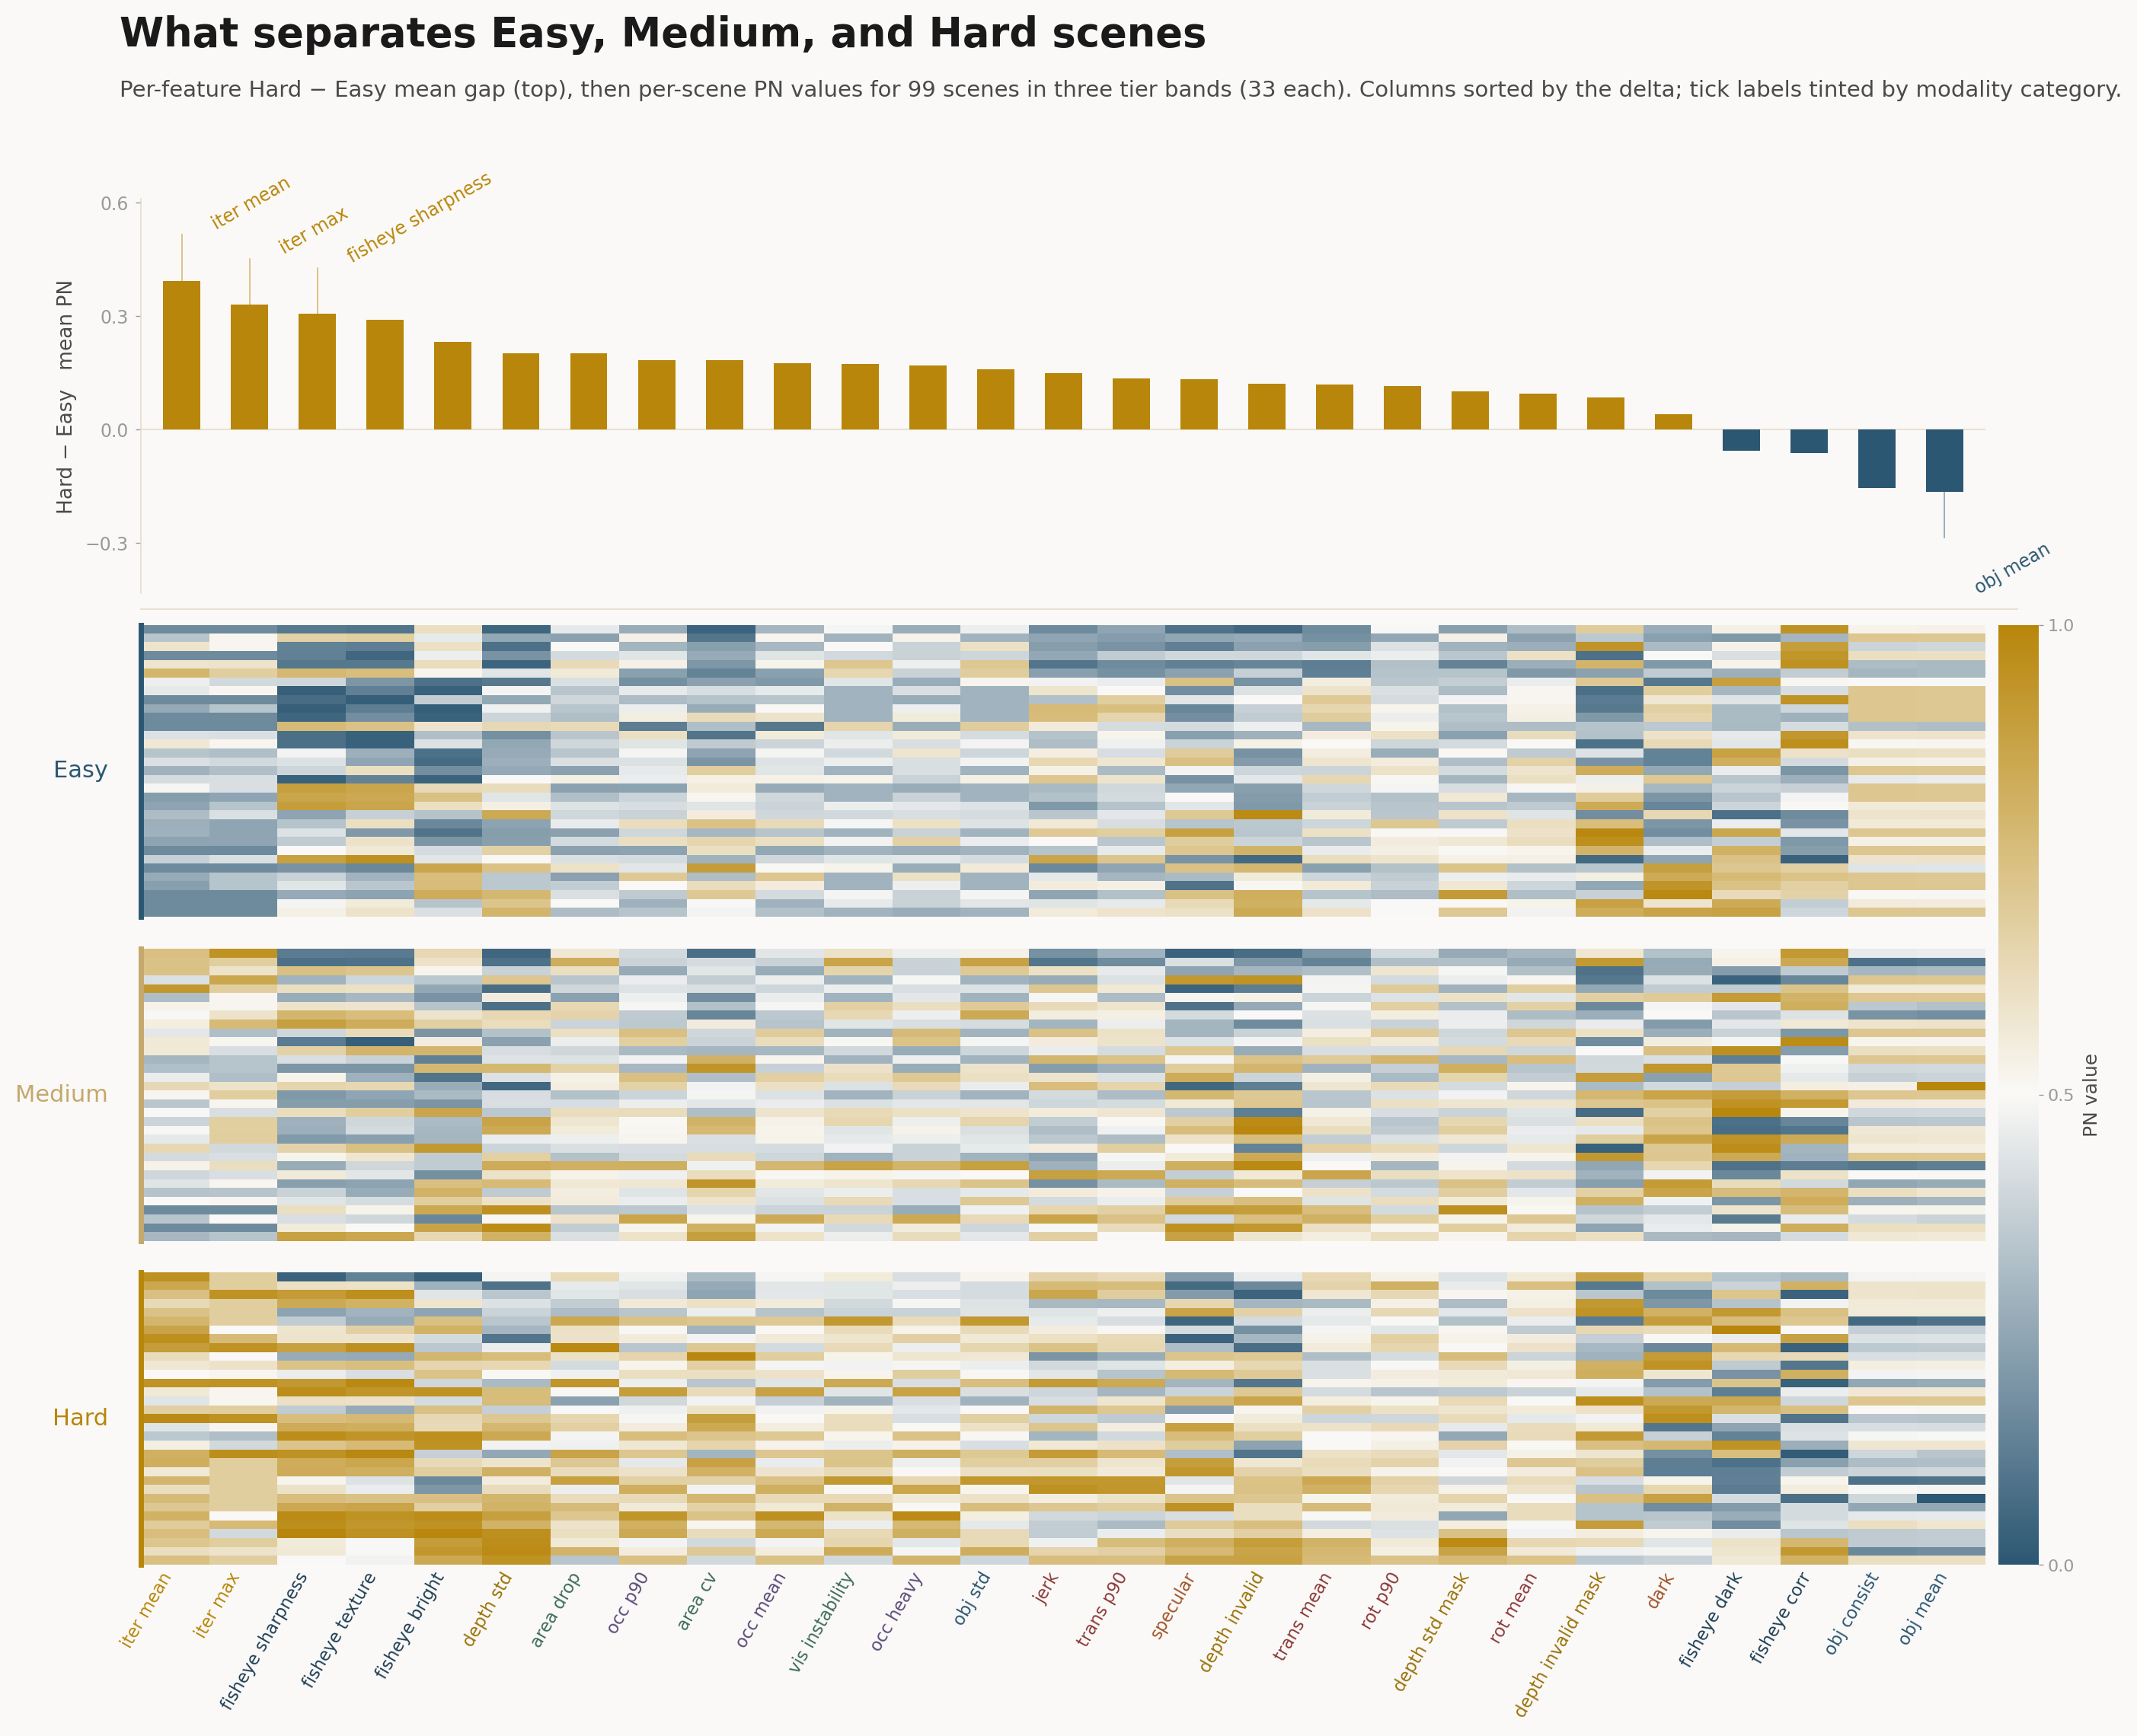
\includegraphics[width=\linewidth]{assets/images/supp_clustermap.png}
\caption{\textbf{What separates Easy, Medium, and Hard scenes.} \emph{Top:} per-feature \textsc{Hard} $-$ \textsc{Easy} mean PN gap, sorted descending. Red bars (positive gap) mark features that are systematically elevated in Hard scenes; teal bars (negative gap) mark features that lean toward Easy. The three most Hard-discriminative features are annotated inline. \emph{Bottom:} per-scene PN values for all 99 scenes, split into three horizontal bands by primary effort\_stratified\_v1 tier (33 scenes each, by tertile cut on the per-scene combined RPX-DS score). Columns are in the same order as the delta bar above; the diverging colormap is centred on the dataset median (0.5), so above-median cells render warm and below-median cells render cool. Visual reading: the Hard band runs warm on the left (where the delta is large and positive) and the Easy band runs cool there, with both bands converging toward the right where the delta crosses zero. X-axis tick labels are tinted by modality category.}
\label{fig:supp-clustermap}
\end{figure}

\begin{figure}[h]
\centering
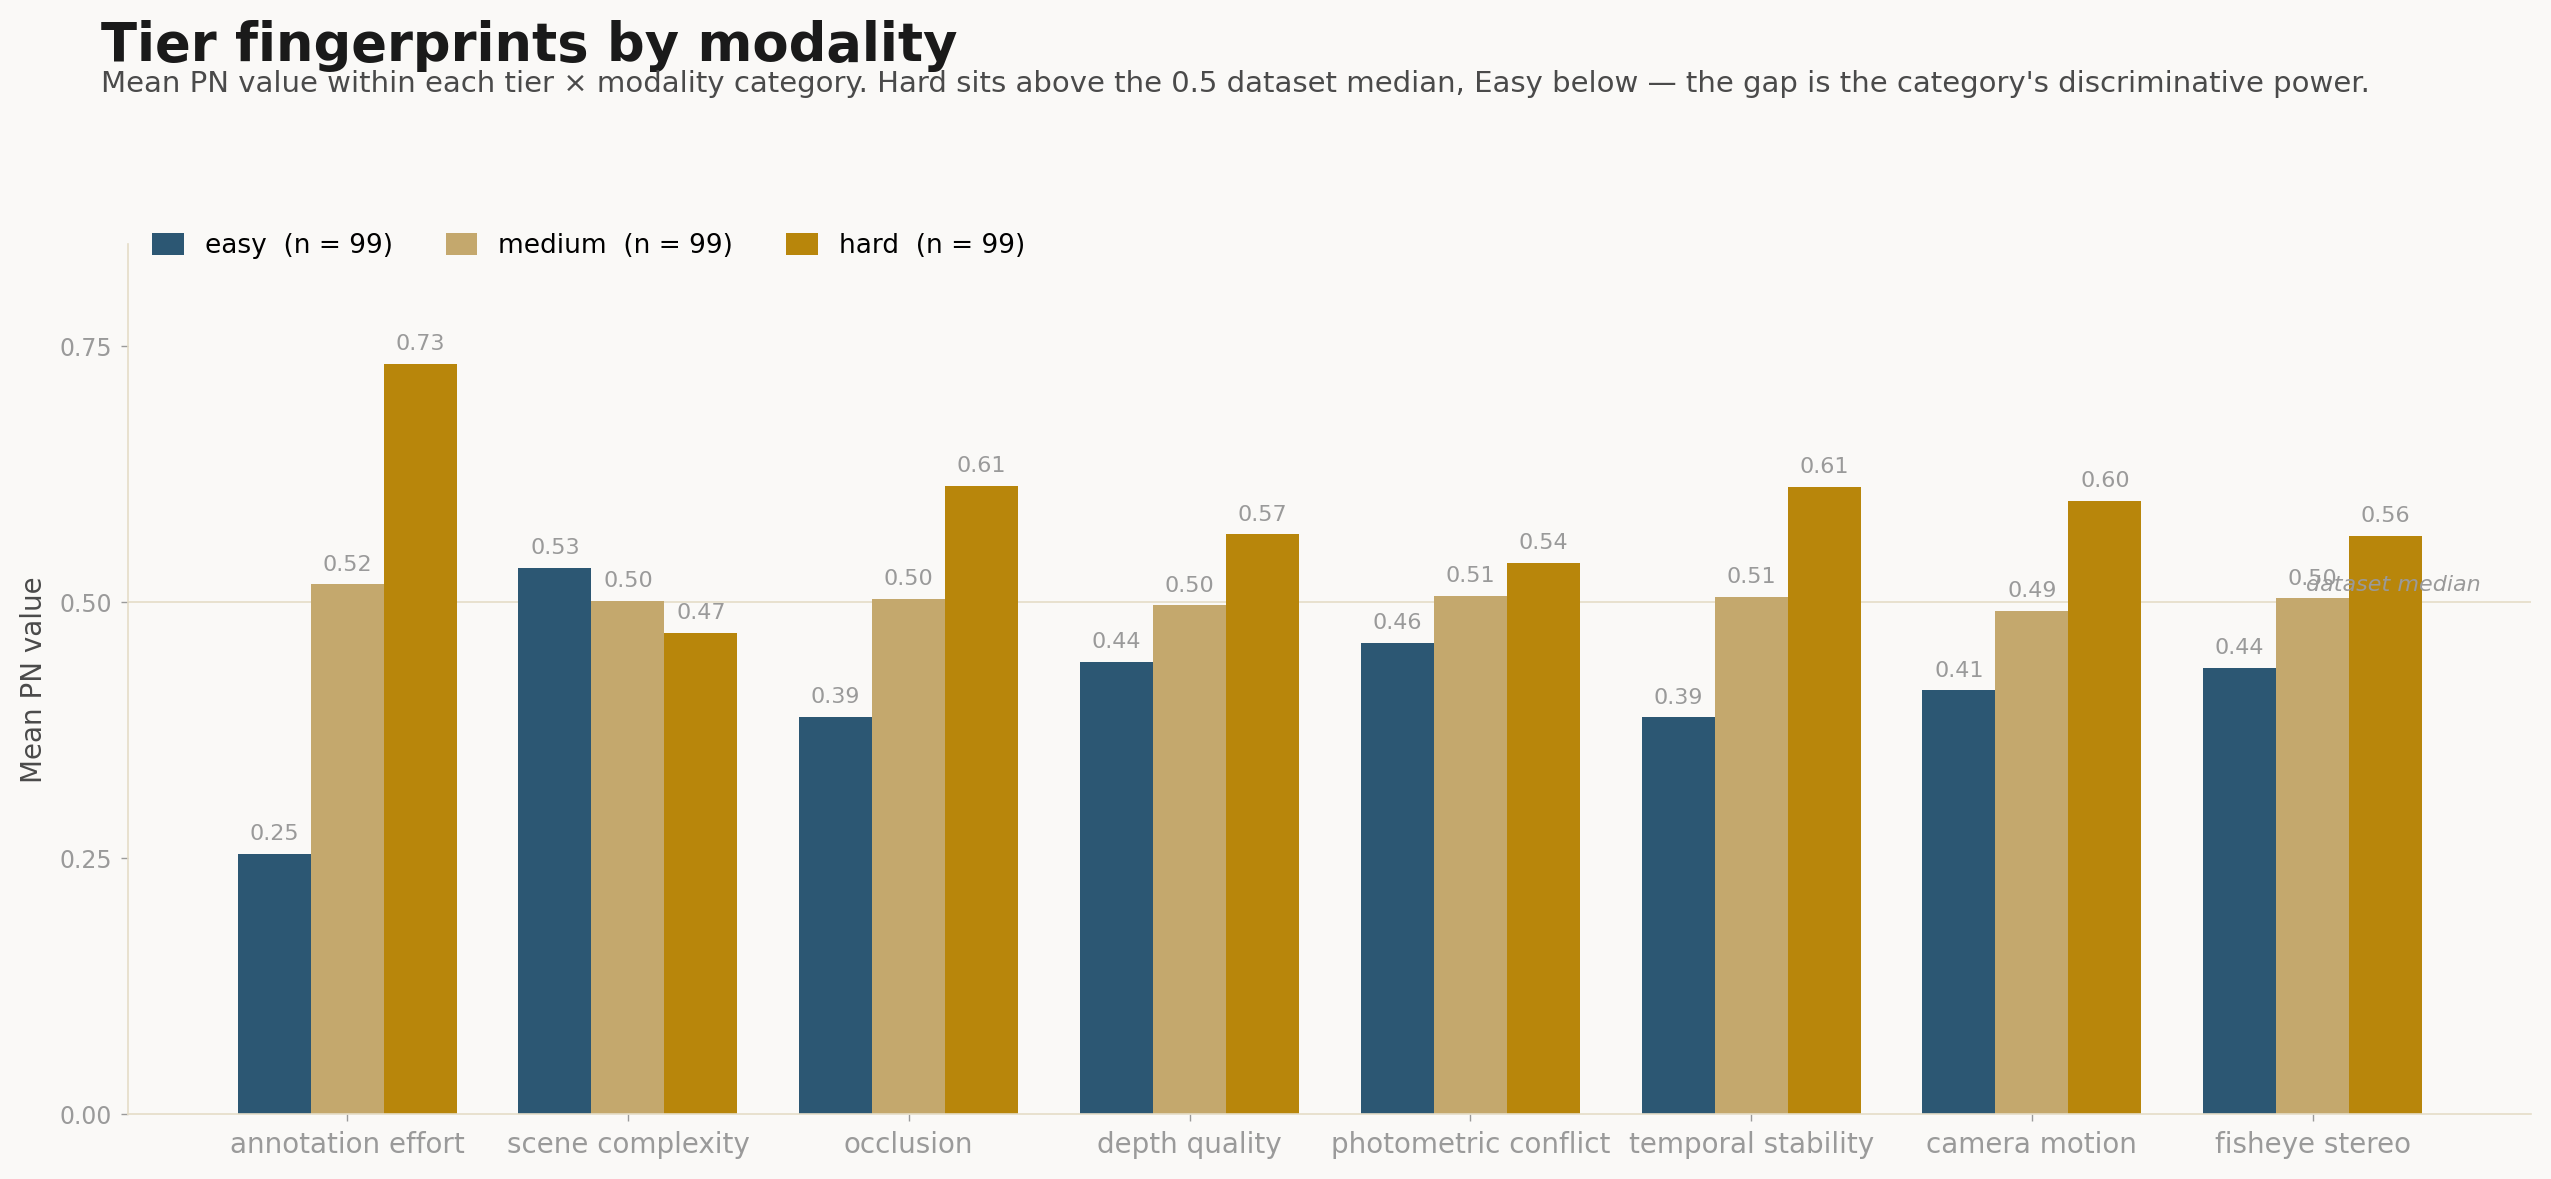
\includegraphics[width=\linewidth]{assets/images/supp_tier_fingerprint.png}
\caption{\textbf{Per-tier fingerprint --- which features pull a scene into each tier.} Mean percentile-normalised feature value within each tier, with the dataset median (0.5) marked. Easy entries (top) sit predominantly below 0.5 across most features; Hard entries (bottom) sit predominantly above 0.5. Annotation-effort features (leftmost two bars, blue) show the largest tier-to-tier swing, which is consistent with the effort-anchored weighting; perception features show the next-largest swings, with depth quality and occlusion notably elevated in the Hard tier.}
\label{fig:supp-tier-fingerprint}
\end{figure}

\begin{figure}[h]
\centering
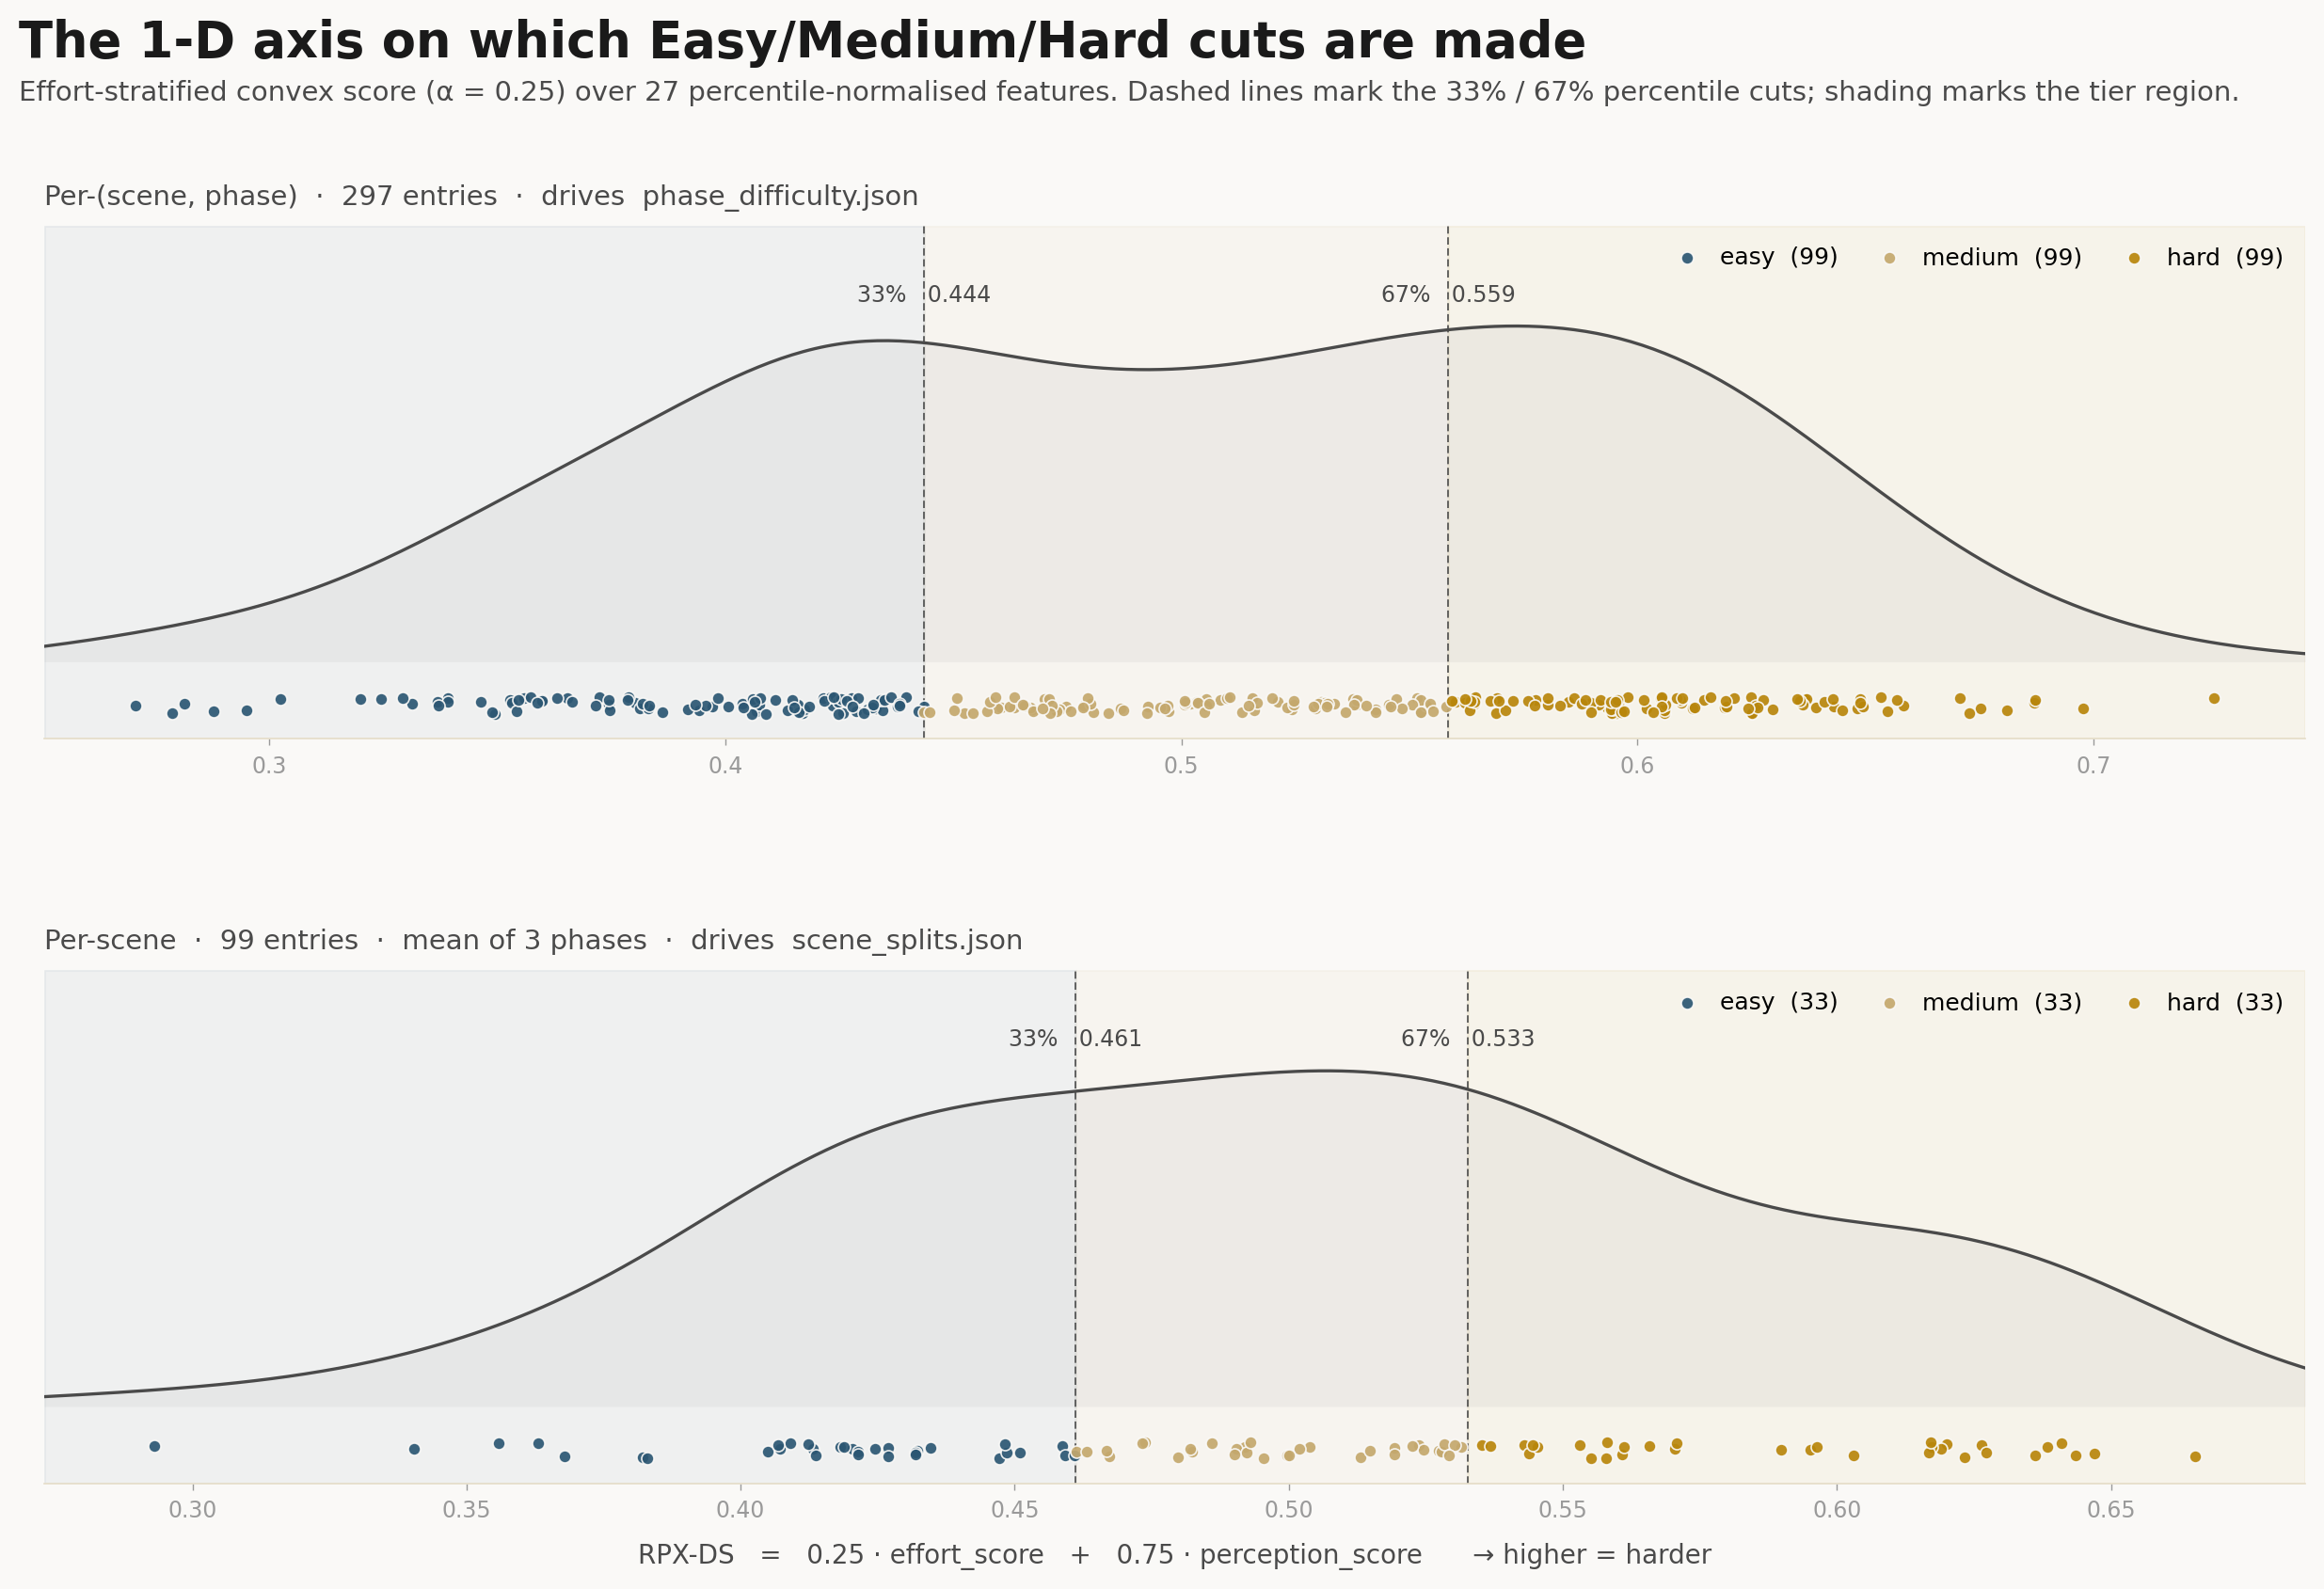
\includegraphics[width=\linewidth]{assets/images/supp_combined_score.png}
\caption{\textbf{The 1-D axis on which Easy/Medium/Hard cuts are made.} The 27-feature percentile-normalised matrix is collapsed to a single scalar via the effort-stratified convex score $\text{RPX-DS}(s,p) = 0.25 \cdot \text{effort\_score} + 0.75 \cdot \text{perception\_score}$, and the 33\% / 67\% percentile cut points (dashed lines) define the Easy / Medium / Hard boundaries. \emph{Top:} per-(scene, phase) view --- 297 entries, the level features are extracted at; tiers here drive \texttt{phase\_difficulty.json}. \emph{Bottom:} per-scene view --- 99 entries, computed as the mean of the 3 per-phase scores per scene; tiers here drive \texttt{scene\_splits.json}. Coloured dots show the assigned tier of each entry; band shading marks the tier region. The per-scene distribution is necessarily tighter than the per-phase one (averaging 3 phases shrinks variance), but the overall unimodal shape and the fact that the cuts sit on relatively gentle slopes --- rather than at sharp valleys --- is what motivates the stability tests in \S\ref{sec:appendix-esd}: small score perturbations near the cuts can flip a few entries' tier assignments without invalidating the global ordering.}
\label{fig:supp-combined-score}
\end{figure}


\section{ESD Weight Sensitivity Analysis}
\label{sec:appendix-esd}

We sample 1{,}000 weight vectors $w$ uniformly from the simplex (Dirichlet$(\mathbf{1})$) over all 27 features and recompute the RPX-DS ranking under each perturbed weight vector.
Compared to the uniform RPX-DS, the median Kendall $\tau$ between the perturbed and uniform rankings is $0.685$ (IQR: $0.630$--$0.734$), demonstrating that the relative difficulty ordering is largely preserved across scoring choices.
At the tier-assignment level, $88.6\%$ of (scene, phase) pairs retain their dominant tier (Easy/Medium/Hard) across the 1{,}000 perturbations; $11.4\%$ of pairs flip tier in fewer than 5\% of perturbations (essentially fully stable), and only $33$ of $297$ pairs ($11.1\%$) flip in more than half of perturbations.
The full per-pair stability table is shipped in the splits manifest (\texttt{benchmark/data/splits/methodology\_study/stability/weight\_perturbation.csv}).


\section{Splits Methodology Study}
\label{sec:appendix-method-study}

To validate the choice of uniform RPX-DS as the primary scoring method, we conducted a seven-layer methodology study comparing 11 scoring methods spanning every major family on the released 297 (scene, phase) feature table.
The study is fully reproducible from the dataset alone (no model results required) and is shipped as \texttt{experiments/neurips-2026/scripts/difficulty\_methodology\_study.py}.

\paragraph{Methods compared.}
\textit{Linear aggregation on percentile-normalised features:} mean (uniform\_v1, our primary), median, max, top-3 mean.
\textit{Dimensionality reduction:} first principal component (PCA-PC1).
\textit{Clustering (mapped to 3 tiers via centroid magnitude):} k-means at $k\in\{3,5,8\}$, Gaussian mixture ($k=3$, full covariance), agglomerative Ward linkage ($k=3$), and DBSCAN with $\epsilon$ chosen via the $k$-distance knee.
For visualisation, we additionally compute t-SNE, Locality Preserving Projections (LPP, \citet{he2003lpp}), and Spectral Embedding 2D projections.

\paragraph{L1: Cross-method agreement.}
Median pairwise Kendall $\tau$ between continuous scores: $0.363$.
Median pairwise Adjusted Rand Index (ARI) between categorical tiers: $0.083$.
Cross-family agreement is generally low---e.g., $\tau(\text{mean\_pn}, \text{max\_pn}) = 0.24$, $\tau(\text{mean\_pn}, \text{PCA-PC1}) = 0.39$---confirming that scoring choice is methodologically consequential and motivating the consensus-tier reporting in \S\ref{sec:features}.

\paragraph{L2: Number of clusters.}
K-means silhouette is maximised at $k=2$ (silhouette $= 0.293$); GMM silhouette is maximised at $k=3$ ($0.238$). Tibshirani's gap statistic also recommends $k=2$ (Fig.~\ref{fig:methstudy-nclusters}).
The data therefore does \textit{not} natively support a 3-cluster structure; the 33/33/34 tertile is adopted as a reporting convention because Easy/Medium/Hard is canonical in benchmarks.

\begin{figure}[h]
\centering
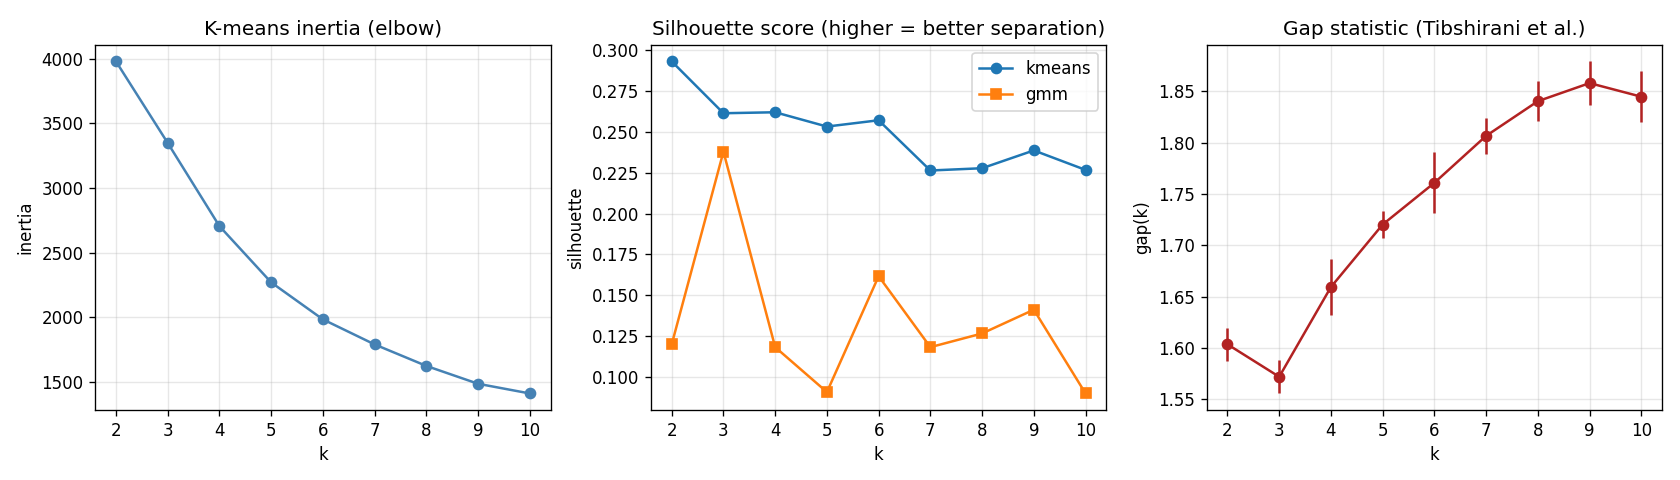
\includegraphics[width=\linewidth]{assets/images/methstudy_n_clusters_diagnostics.png}
\caption{\textbf{Cluster-count diagnostics on the 297-pair, 27-feature matrix.} K-means inertia (left) shows no sharp elbow. K-means silhouette (centre, blue) peaks at $k=2$; GMM silhouette (centre, orange) peaks at $k=3$. Tibshirani's gap statistic (right) is monotonically increasing through $k=10$; the smallest $k$ satisfying gap$(k) \geq$ gap$(k+1) - s_{k+1}$ is $k=2$. The data does not natively prefer $k=3$ — the tertile is a reporting convention.}
\label{fig:methstudy-nclusters}
\end{figure}

\paragraph{L3: Stability under perturbations.}
Three independent perturbation studies on uniform\_v1 (1{,}000 iterations each unless noted):
\textit{(a) Bootstrap subsampling (80\%):} median per-pair dominant-tier stability $= 1.000$; $89.9\%$ of pairs have $>$95\% stability across resamples; $81.1\%$ of pairs are perfectly stable.
\textit{(b) Weight perturbation (Dirichlet$(\mathbf{1})$):} median tier-flip rate $0.348$; $88.6\%$ of pairs retain dominant tier (see \S\ref{sec:appendix-esd} for the full Kendall-$\tau$ analysis).
\textit{(c) Feature dropout (drop 1/3 random features, 200 iterations):} median tier-flip rate $0.275$; $23.9\%$ of pairs flip in $<$5\% of dropouts.
The full per-pair distributions are in Fig.~\ref{fig:methstudy-stability}.

\begin{figure}[h]
\centering
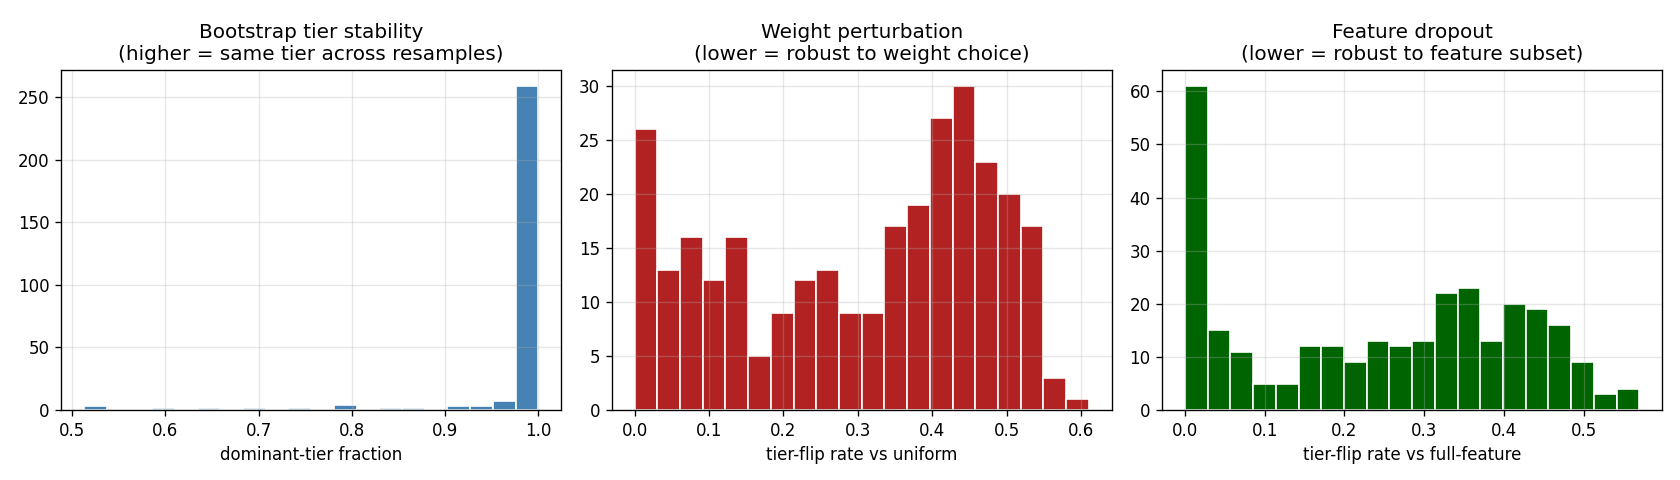
\includegraphics[width=\linewidth]{assets/images/methstudy_stability_distribution.png}
\caption{\textbf{Stability of the uniform\_v1 tier assignment under three perturbation studies.} Bootstrap subsampling (left, blue) is dominated by the mass at 1.0 — the assignment is essentially invariant to which 80\% of scenes is sampled. Weight perturbation (centre, red) is bimodal: a stable subpopulation flips little and a sensitive subpopulation flips ${\sim}50\%$ of the time. Feature dropout (right, green) shows a stable mode at 0 and a long tail. Bootstrap-rock-stable but weight-sensitive — the case for shipping the consensus tier alongside any single primary method.}
\label{fig:methstudy-stability}
\end{figure}

\paragraph{L4: Outliers.}
Twelve (scene, phase) pairs exceed the $\chi^2_{27}(0.99)$ Mahalanobis-distance threshold in the percentile-normalised feature space. The top entries by distance are \texttt{scene100.jsom.atrium} interaction phase ($d=11.95$), \texttt{scene18.su.CHECKERBOARD} clutter phase ($d=10.86$), and \texttt{scene74.ecsw.atriumStairs} clean phase ($d=7.69$). Two of these (\texttt{scene100} and \texttt{scene74}) coincide with documented T265 tracking-failure events during capture, demonstrating that the methodology surfaces genuine data quality issues from the feature distribution alone.

\paragraph{L5: Cross-method consensus.}
Across the 11 methods (DBSCAN excluded as degenerate---it found no density modes in the 27D feature space), only $24$ of $297$ pairs ($8.1\%$) receive unanimous tier assignment. $104$ pairs ($35.0\%$) are split between two tiers, and $169$ pairs ($56.9\%$) span all three (Fig.~\ref{fig:methstudy-consensus}).
The consensus tier (majority vote) is shipped alongside uniform\_v1 in the splits manifest.

\begin{figure}[h]
\centering
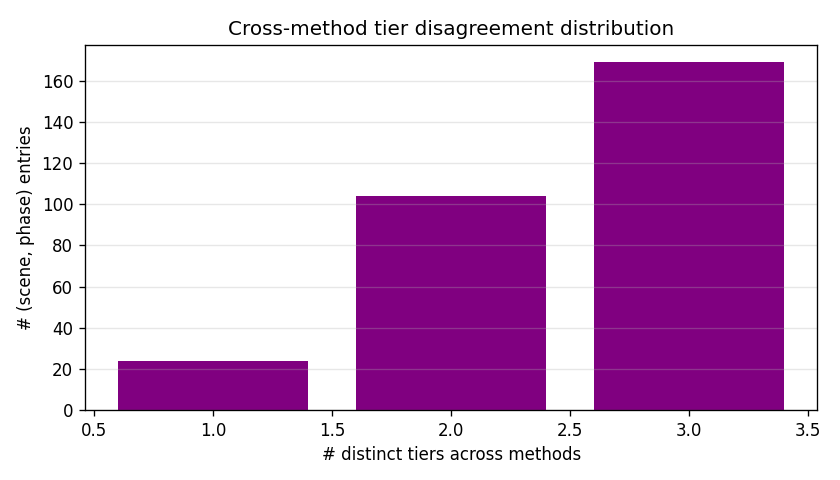
\includegraphics[width=0.55\linewidth]{assets/images/methstudy_consensus_disagreement.png}
\caption{\textbf{Cross-method tier disagreement.} Histogram of distinct tiers assigned per (scene, phase) across 11 scoring methods. Only 8.1\% of pairs receive unanimous agreement; the majority span 2 or 3 tiers. The consensus tier (majority vote) is shipped alongside the primary uniform\_v1 tier.}
\label{fig:methstudy-consensus}
\end{figure}

\paragraph{L6: Phase signature.}
The maximum ARI between any clustering method's labels and the capture-phase index (clutter/interaction/clean) is $0.182$ (k-means at $k=8$); for $k=3$ partitions specifically: k-means $0.177$, GMM $0.036$, Ward $0.003$, DBSCAN $0.003$. Feature space therefore captures perception difficulty rather than capture-protocol identity---validating that ESD splits are a difficulty stratification, not a phase classifier.

\paragraph{Per-feature contribution by tier.}
Fig.~\ref{fig:methstudy-features} shows the mean percentile-normalised value of each feature within each Easy/Medium/Hard tier. Hard scenes are higher than Easy on most features---confirming the score is broadly difficulty-tracking rather than driven by a single modality. Three features show inverted ordering: $f_{\text{obj-mean}}$ and $f_{\text{obj-consist}}$ (densely-arranged static scenes are ``Easy'' in the multi-feature sense), and $f_{\text{fisheye-corr}}$ (transparent or motion-blurred scenes break stereo correlation, marking them as Hard with low corr).

\begin{figure}[h]
\centering
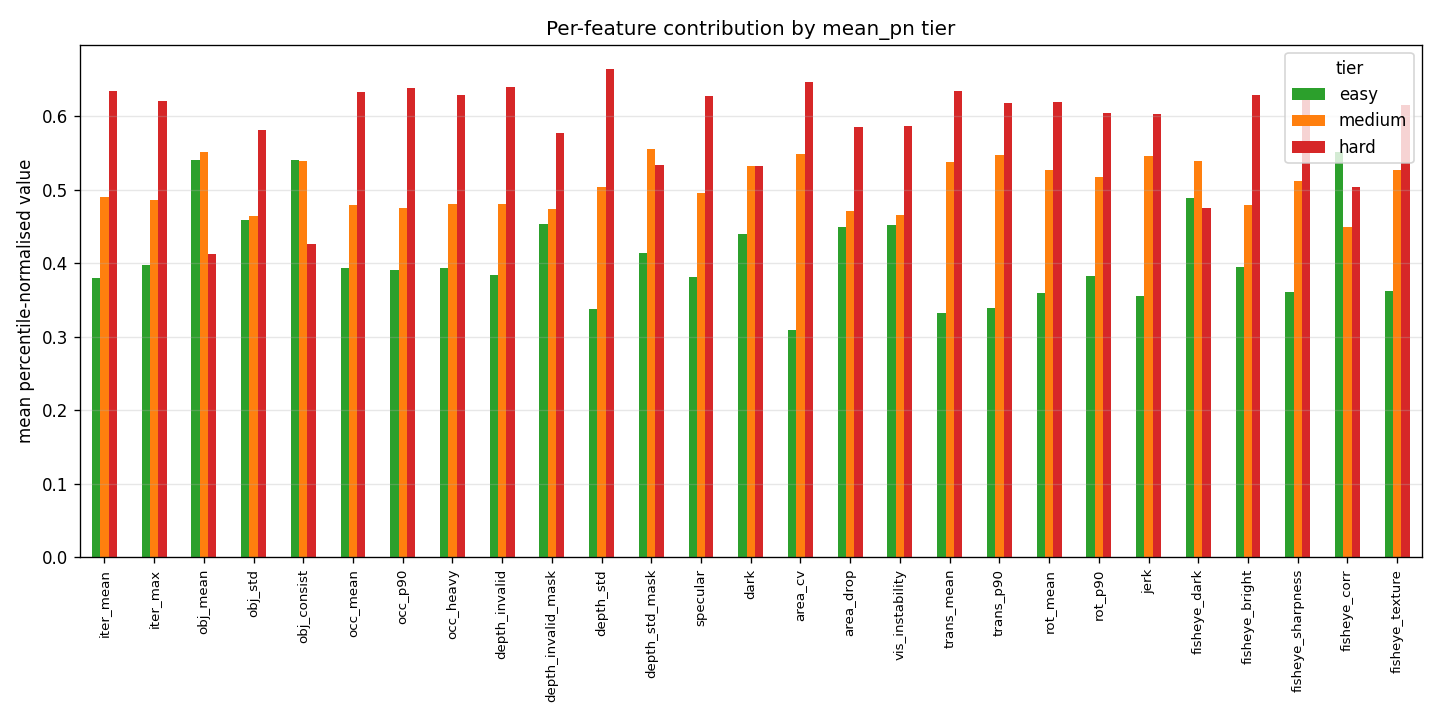
\includegraphics[width=\linewidth]{assets/images/methstudy_feature_contributions_by_tier.png}
\caption{\textbf{Per-feature mean percentile-normalised value by uniform\_v1 tier.} Hard tier (red) is uniformly higher than Easy (green) on most features, confirming the multi-modal nature of the difficulty signal. Three inversions ($f_{\text{obj-mean}}$, $f_{\text{obj-consist}}$, $f_{\text{fisheye-corr}}$) reveal that scene complexity ${\neq}$ scene difficulty: densely arranged but well-lit static scenes can still be Easy, while sparsely arranged but transparent or moving scenes are Hard.}
\label{fig:methstudy-features}
\end{figure}

\paragraph{Reproducibility.}
All numbers above are deterministic given seed=0; the full study (tables, plots, and per-entry assignments under all 11 methods) ships under \texttt{benchmark/data/splits/methodology\_study/}, with input file SHA-256 stamped into \texttt{provenance.json}.


\section{Ground-Truth Annotation Pipeline}
\label{sec:appendix-annotation}

This section documents the three major annotation pipelines in detail.
Figure~\ref{fig:mask-pipeline} illustrates the mask annotation workflow,
Figure~\ref{fig:qa-generation} illustrates the QA ground-truth generation,
and Figure~\ref{fig:pose-refinement} illustrates the camera pose refinement procedure.

\subsection{Instance Mask Annotation}
\label{sec:appendix-masks}

\begin{figure}[h]
    \centering
    % \includegraphics[width=\linewidth]{assets/images/mask-pipeline.pdf}
    \todo{Figure: mask annotation pipeline diagram — SAM2 auto $\to$ GroundingDINO bbox proposals $\to$ human iterative refinement UI $\to$ final masks. Show example frames at each stage.}
    \caption{Instance mask annotation pipeline. (1)~SAM2 auto-mode generates initial masks.
    (2)~GroundingDINO proposes bounding boxes for missed objects using text prompts from the object questionnaire.
    (3)~A human annotator iteratively refines boundaries in a custom UI until sub-pixel accuracy at object edges.
    The refinement iteration count $k_j$ per instance feeds ESD (\S\ref{sec:features}).}
    \label{fig:mask-pipeline}
\end{figure}

SAM2~\citep{ravi2024sam2} in automatic mode generates initial instance masks for each keyframe.
GroundingDINO~\citep{liu2024groundingDINO} provides complementary bounding-box proposals using per-object category names from the FewSOL questionnaire, catching objects that SAM2's class-agnostic mode misses (e.g.\ transparent items, thin utensils).
A custom annotation interface then enables iterative human refinement: annotators adjust mask boundaries, split merged instances, and add missing objects until edges align with object contours at sub-pixel accuracy.
The refinement iteration count $k_j$ per instance is recorded and directly feeds the ESD difficulty model (Section~\ref{sec:features})---scenes requiring more human correction are empirically harder for models.

\paragraph{Tracklets.}
SAM2 video propagation with human-corrected keyframe initialisation produces dense tracklets with consistent IDs across each phase.
Annotators verify ID consistency at phase boundaries and correct drift or ID switches introduced by fast hand motion during interaction.

\subsection{QA Ground-Truth Generation}
\label{sec:appendix-qa}

\begin{figure}[h]
    \centering
    % \includegraphics[width=\linewidth]{assets/images/qa-generation.pdf}
    \todo{Figure: QA generation pipeline — (a) human-authored template bank with robotics-grounded question types, (b) per-frame instantiation using visibility masks + bbox geometry + questionnaire attributes, (c) example Q/A pairs showing phase-varying answers.}
    \caption{QA ground-truth generation. Humans author question templates grounded in robotics operator needs (left).
    Templates are instantiated deterministically per frame using object visibility masks, bounding-box geometry, and questionnaire attributes (centre).
    The same question produces different correct answers across phases (right).}
    \label{fig:qa-generation}
\end{figure}

\paragraph{Template design.}
A set of question templates was authored by hand to reflect the information needs of a robot operator or planner.
Templates fall into four categories:
\textbf{(i)~Identity}: ``What objects are on the table?'', ``Is there a \{category\}?'';
\textbf{(ii)~Attribute verification}: ``What colour is the \{object\}?'', ``What material is the \{object\}?'';
\textbf{(iii)~Counting}: ``How many objects are visible?'';
\textbf{(iv)~Spatial relations} (D5): ``What is to the left/right/above/below of the \{object\}?''.
All templates use crowd-sourced natural-language object descriptions from FewSOL questionnaires~\citep{padalunkal2023fewsol} (\S\ref{sec:dataset}), matching how real users command robots.

\paragraph{Instantiation.}
For each frame $t$, templates are instantiated deterministically:
(a)~per-frame visibility is determined from instance masks (an object is ``visible'' if its mask area exceeds a minimum threshold);
(b)~identity and attribute answers are read from the questionnaire;
(c)~spatial relations are computed in the \textit{image plane} using polar coordinates centred on the reference object's bounding-box centroid.
This yields \todo{X} Q/A pairs per scene across all phases.
Critically, the same question has \textit{different correct answers} across phases (e.g.\ objects are rearranged, new objects become visible), making this, to our knowledge, the first perception QA benchmark with phase-varying ground truth.

\paragraph{Spatial relation definition.}
All spatial relations are defined in the image plane: ``left'' = centroid with smaller $x$-coordinate; ``above'' = smaller $y$-coordinate; ``near'' = Euclidean distance $<\tau_\text{near}$ pixels.
This matches how VLMs process images and avoids ambiguity from world-frame perspective.

\subsection{Camera Pose Refinement}
\label{sec:appendix-pose}

\begin{figure}[h]
    \centering
    % \includegraphics[width=\linewidth]{assets/images/pose-refinement.pdf}
    \todo{Figure: pose refinement pipeline — T265 raw VIO trajectory $\to$ outlier rejection $\to$ optional loop closure $\to$ refined trajectory. Show before/after trajectory overlay on a sample scene.}
    \caption{Camera pose refinement. Raw T265 VIO at 200\,Hz is downsampled to 30\,fps,
    filtered for outlier jumps, and validated via loop-closure analysis on closed-loop sequences.}
    \label{fig:pose-refinement}
\end{figure}

T265 VIO provides 6-DoF camera pose at 200\,Hz, downsampled to 30\,fps to align with D435 frames.
Raw T265 odometry is used as the pose reference---no offline bundle adjustment is applied, preserving the noise profile that deployed robots would encounter with the same sensor.
Over ${\sim}$250 frames (${\sim}$8\,s per phase), drift is bounded to $<$\todo{X}\,cm / $<$\todo{X}$^\circ$ via loop-closure analysis on \todo{N} closed-loop sequences where the camera returns to its starting position.
Outlier frames with $\Delta t > \todo{X}$\,cm or $\Delta R > \todo{X}^\circ$ between consecutive frames are flagged and excluded from temporal stability (TS) computation.

\paragraph{Depth ground truth.}
Raw D435 structured-light depth; invalid pixels (specular reflection, transparency, range limits) are flagged and excluded from evaluation.
No inpainting is applied---models are evaluated only on pixels where the sensor produces valid returns.

\paragraph{Language annotations.}
Per-object attributes (category, colour, material, shape) from FewSOL~\citep{padalunkal2023fewsol} questionnaires serve as referring expressions for grounding evaluation and as the vocabulary source for QA template instantiation (\S\ref{sec:appendix-qa}).


\section{Per-Task Detailed Results}
\label{sec:appendix-per-task}

% ── TODO(results): one table per task with full breakdowns ──
\todo{One table per task (D1--D5) with:
All models (including appendix-only: DA-V2 Base, Prompt DA, MiDaS, SAM2 Small, DITO, RO-ViT, etc.).
Per-ESD columns (Easy / Medium / Hard).
Per-phase columns ($\mathcal{P}_{\text{clu}}$ / $\mathcal{P}_{\text{int}}$ / $\mathcal{P}_{\text{cln}}$).
Full metric suite (not just primary metric).
Params, FLOPs, median latency.}


\section{Camera Motion Statistics}
\label{sec:appendix-motion}

% ── TODO(data): compute from T265 poses ──
\todo{Full-page figure:
(a) Histogram of $\Delta t$ (cm/frame) across 100 scenes $\times$ 3 phases.
(b) Histogram of $\Delta R$ (deg/frame).
(c) Histogram of jerk.
(d) Overlay with published platform motion profiles from Stretch RE2, Unitree H1, Fetch, Spot.}


\section{Dataset Object Taxonomy}
\label{sec:appendix-objects}

% ── TODO(data): compile from annotation metadata ──
\todo{Full object taxonomy:
$\sim$70 categories with supercategory assignments, instance counts, YCB/FewSOL overlap markers.
Example images.}


\section{Text vs.\ Visual Prompting: Extended Analysis}
\label{sec:appendix-prompting}

% ── TODO(results): extended D3 analysis ──
\todo{Extended comparison of text-prompted (GroundingDINO, OWL-ViT, YOLO-World, Qwen2-VL)
vs.\ image-prompted (DE-ViT, NIDS-Net, Qwen2-VL with visual prompt) detection.
Per-ESD, per-phase breakdown.
Analysis of which object categories benefit most from each prompting mode.
Failure case examples: text prompt fails when spatial relations change; visual prompt fails under viewpoint shift.}


\section{\coolname{} Toolkit: Extended Documentation}
\label{sec:appendix-toolkit}

This appendix provides extended documentation for the \texttt{rpx-benchmark} toolkit described in Section~\ref{sec:toolkit}.

\paragraph{Python API usage example.}
\begin{verbatim}
from rpx_benchmark import (
    RPXDataset, BenchmarkRunner,
    MetricSuite, TaskType
)

dataset = RPXDataset.from_manifest("rpx_test.json")
model   = MyDepthModel()  # subclasses BenchmarkModel
suite   = MetricSuite.for_task(TaskType.MONOCULAR_DEPTH)
runner  = BenchmarkRunner(model, dataset, suite)

result, dr = runner.run_with_deployment_readiness(
    primary_metric="abs_rel",
    model_name="MyDepthModel"
)
print(dr.summary())
\end{verbatim}

The \texttt{dr.summary()} output:
\begin{verbatim}
--- RPX Deployment Readiness: MyDepthModel ---
  S_overall  = 0.134 (AbsRel, lower=better)
  STR_{C->I} = -0.023 (interaction drop)
  STR_{I->L} = +0.018 (recovery)
  TS         = 0.891 (temporal stability)
  SGC        = 0.672 (geometric coherence)
  Params     = 335M   FLOPs = 211G
  Latency    = 45ms (median, per frame)
\end{verbatim}

\paragraph{Adding a new task.}
\begin{verbatim}
from rpx_benchmark.tasks import register_task, TaskSpec
register_task(TaskSpec(
    name="affordance_prediction",
    runner=my_affordance_runner,
    metrics=["auc", "f1"],
    input_modalities=["rgb", "depth"],
))
\end{verbatim}

\paragraph{Adding a new metric.}
\begin{verbatim}
from rpx_benchmark.metrics import BaseMetric, register_metric
class GraspAlignment(BaseMetric):
    def compute(self, pred_mask, gt_depth):
        return score
register_metric("grasp_alignment", GraspAlignment)
\end{verbatim}

\paragraph{CI.} 138 offline tests, Python 3.10/3.11/3.12, GitHub Actions, zero network deps.
MkDocs + mkdocstrings auto-docs. Ruff lint.


\section{Cross-Task Ranking Agreement}
\label{sec:appendix-cross-task}

% ── TODO(analysis): cross-task correlation ──
\todo{(a) Kendall $\tau$ of $S_\text{overall}$ rankings for task pairs sharing $\geq$2 models.
(b) Kendall $\tau$ of scene difficulty rankings across tasks (ESD consistency).
(c) For shared-backbone models: does deployment readiness transfer across tasks?}


\section{Croissant Metadata and Datasheet}
\label{sec:appendix-croissant}

\coolname{} is documented using Croissant~\citep{akhtar2024croissant} with core and RAI fields, as required by NeurIPS 2026 E\&D Track.
\textbf{Core:} name, URL, licence (CC BY 4.0), format, record sets for each modality.
\textbf{RAI:} collection protocol, consent, PII assessment (none), annotation methodology, known biases (indoor-dominant, D435 range, human motion profile).
The Croissant JSON is included with the supplementary materials and hosted on HuggingFace.

\section{Scope, Assumptions, and Output-vs-Feature Evaluation}
\label{sec:appendix-scope}

\coolname{} is designed to test the claim: \textit{pretrained perception backbones differ in deployment robustness, and this difference is not predictable from standard accuracy alone.}

\paragraph{Output-level vs.\ feature-level evaluation.}
Robot learning systems consume perception at two levels.
\textbf{(a)~As raw signals:} modular systems (OK-Robot, DP3, AnyGrasp~\citep{liu2024okrobot, ze2024dp3}) directly consume depth maps, bounding boxes, and masks---for these, \coolname{} evaluates the signal the robot directly consumes.
\textbf{(b)~As encoded features:} VLAs ($\pi_0$, OpenVLA, GR00T) consume frozen or fine-tuned encoder activations, never producing an explicit depth map or detection.
For these, \coolname{}'s task-level metrics serve as \textit{proxies} for feature quality: a backbone whose outputs exhibit low temporal stability (TS) or poor phase-transition robustness (STR) has representations that fail to stably encode scene geometry or handle occlusion, and an action-conditioned decoder is unlikely to fully recover information the encoder failed to capture.
Furthermore, \coolname{}'s VLM evaluation (D4/D5) directly tests the same VLMs (PaliGemma, Qwen2-VL) that VLAs are built on.
The downstream validation in \S\ref{sec:downstream} empirically tests whether \coolname{}'s rankings transfer to task-level success.

\paragraph{Additional assumptions.}
(i)~Human-carried capture is a valid motion proxy (validated in \S\ref{sec:dataset} and Appendix~\ref{sec:appendix-motion}).
(ii)~100 scenes are representative of deployment environments.
(iii)~Zero-shot evaluation reflects deployment conditions.

\paragraph{Out of scope.}
Navigation-specific perception, sensing outside the D435/T265 envelope (0.3--3\,m indoor + matched outdoor), and platforms with non-humanoid kinematics (e.g., fixed-base arms with restricted viewpoints).



\newpage
\section*{NeurIPS Paper Checklist}

\begin{enumerate}

\item {\bf Claims}
    \item[] Question: Do the main claims made in the abstract and introduction accurately reflect the paper's contributions and scope?
    \item[] Answer: \answerYes{}
    \item[] Justification: The abstract and introduction state that \coolname{} is a unified RGB-D benchmark with five perception tasks, three-phase capture, and ESD-stratified difficulty splits. Sections~\ref{sec:dataset}--\ref{sec:experiments} directly support each claim with dataset statistics, metric definitions, and experimental results. Scope limitations (indoor-only, D435 depth range, human-driven capture trajectories) are stated in Section~\ref{sec:dataset} and the conclusion.

\item {\bf Limitations}
    \item[] Question: Does the paper discuss the limitations of the work performed by the authors?
    \item[] Answer: \answerYes{}
    \item[] Justification: The conclusion contains a dedicated \emph{Limitations} paragraph discussing T265 odometry drift, D435 depth range constraints, indoor-only capture, and annotator diversity. The dataset card (Croissant) repeats these.

\item {\bf Theory assumptions and proofs}
    \item[] Question: For each theoretical result, does the paper provide the full set of assumptions and a complete (and correct) proof?
    \item[] Answer: \answerNA{}
    \item[] Justification: The paper presents an empirical benchmark and dataset; it contains no theoretical results or proofs.

    \item {\bf Experimental result reproducibility}
    \item[] Question: Does the paper fully disclose all the information needed to reproduce the main experimental results of the paper to the extent that it affects the main claims and/or conclusions of the paper (regardless of whether the code and data are provided or not)?
    \item[] Answer: \answerYes{}
    \item[] Justification: The evaluation toolkit is pip-installable (\texttt{rpx-benchmark}), open-source (MIT), and includes a continuous-integration test suite verifying reproducibility of all metric computations. Sensor specifications, annotation protocol details, and evaluation setup are described in Sections~\ref{sec:dataset} and~\ref{sec:tasks}. All model checkpoints are public.

\item {\bf Open access to data and code}
    \item[] Question: Does the paper provide open access to the data and code, with sufficient instructions to faithfully reproduce the main experimental results, as described in supplemental material?
    \item[] Answer: \answerYes{}
    \item[] Justification: The dataset is hosted on HuggingFace Datasets under CC BY 4.0 with a 5-scene reviewer sample available without registration. The evaluation toolkit source code is publicly available under the MIT licence with pip-installable dependencies and a documented CLI.

\item {\bf Experimental setting/details}
    \item[] Question: Does the paper specify all the training and test details (e.g., data splits, hyperparameters, how they were chosen, type of optimizer) necessary to understand the results?
    \item[] Answer: \answerYes{}
    \item[] Justification: Section~\ref{sec:dataset} describes the train/val/test splits (70/15/15 scenes, no overlap), Section~\ref{sec:features} defines ESD computation and thresholds, and Section~\ref{sec:experiments} reports GPU type, inference settings, and per-model checkpoint identifiers. No training or fine-tuning is performed; all models are evaluated zero-shot.

\item {\bf Experiment statistical significance}
    \item[] Question: Does the paper report error bars suitably and correctly defined or other appropriate information about the statistical significance of the experiments?
    \item[] Answer: \answerYes{}
    \item[] Justification: Tables report standard deviation across scenes alongside mean values. The ESD sensitivity analysis (Appendix~A) uses 1{,}000 Monte Carlo weight perturbations to assess split stability.

\item {\bf Experiments compute resources}
    \item[] Question: For each experiment, does the paper provide sufficient information on the computer resources (type of compute workers, memory, time of execution) needed to reproduce the experiments?
    \item[] Answer: \answerYes{}
    \item[] Justification: Section~\ref{sec:experiments} states GPU type, VRAM, and per-model inference time. The toolkit automatically reports FLOPs and median per-sample latency in every run.

\item {\bf Code of ethics}
    \item[] Question: Does the research conducted in the paper conform, in every respect, with the NeurIPS Code of Ethics \url{https://neurips.cc/public/EthicsGuidelines}?
    \item[] Answer: \answerYes{}
    \item[] Justification: The dataset contains indoor daily objects; no faces, biometric identifiers, or personally identifiable information are captured. All capture was performed by lab personnel who provided informed consent for data release. The work does not raise dual-use concerns.

\item {\bf Broader impacts}
    \item[] Question: Does the paper discuss both potential positive societal impacts and negative societal impacts of the work performed?
    \item[] Answer: \answerYes{}
    \item[] Justification: The conclusion includes a \emph{Broader Impact} paragraph discussing both the positive impact (enabling safer robot deployment through rigorous perception evaluation) and the limited risk profile (indoor daily-object scenes with no misuse pathway).

\item {\bf Safeguards}
    \item[] Question: Does the paper describe safeguards that have been put in place for responsible release of data or models that have a high risk for misuse (e.g., pre-trained language models, image generators, or scraped datasets)?
    \item[] Answer: \answerNA{}
    \item[] Justification: The dataset contains only indoor tabletop scenes with daily objects. It does not contain faces, personal data, generative models, or any content that poses a misuse risk.

\item {\bf Licenses for existing assets}
    \item[] Question: Are the creators or original owners of assets (e.g., code, data, models), used in the paper, properly credited and are the license and terms of use explicitly mentioned and properly respected?
    \item[] Answer: \answerYes{}
    \item[] Justification: All evaluated models are cited with their original publications and checkpoint sources. The dataset is released under CC BY 4.0; the toolkit under MIT. Overlap with YCB and FewSOL object sets is acknowledged with citations.

\item {\bf New assets}
    \item[] Question: Are new assets introduced in the paper well documented and is the documentation provided alongside the assets?
    \item[] Answer: \answerYes{}
    \item[] Justification: The dataset is accompanied by a Croissant metadata file (machine-readable dataset card), a HuggingFace dataset card, and the \texttt{rpx-benchmark} toolkit with auto-generated API documentation from source-level docstrings. The collection protocol, consent details, privacy considerations, and known biases are documented in the dataset card.

\item {\bf Crowdsourcing and research with human subjects}
    \item[] Question: For crowdsourcing experiments and research with human subjects, does the paper include the full text of instructions given to participants and screenshots, if applicable, as well as details about compensation (if any)?
    \item[] Answer: \answerYes{}
    \item[] Justification: Data capture and annotation were performed by lab personnel (not crowdsourced). The annotation protocol (SAM2 auto-masks with iterative human refinement) is described in Section~\ref{sec:dataset}. All participants provided informed consent for data collection and public release.

\item {\bf Institutional review board (IRB) approvals or equivalent for research with human subjects}
    \item[] Question: Does the paper describe potential risks incurred by study participants, whether such risks were disclosed to the subjects, and whether Institutional Review Board (IRB) approvals (or an equivalent approval/review based on the requirements of your country or institution) were obtained?
    \item[] Answer: \answerNA{}
    \item[] Justification: The study involves only video capture of tabletop objects and human hands during manipulation. No experimental interventions on human subjects were conducted. Participants are lab members who consented to hand appearance in the interaction-phase recordings.

\item {\bf Declaration of LLM usage}
    \item[] Question: Does the paper describe the usage of LLMs if it is an important, original, or non-standard component of the core methods in this research? Note that if the LLM is used only for writing, editing, or formatting purposes and does \emph{not} impact the core methodology, scientific rigor, or originality of the research, declaration is not required.
    \item[] Answer: \answerNA{}
    \item[] Justification: LLMs are not part of the core method. LLMs were used only for writing assistance and code generation during toolkit development, which does not impact the scientific methodology or experimental results.

\end{enumerate}


\end{document}
